\documentclass[12pt]{article}
\setlength{\oddsidemargin}{-0.125in}
\setlength{\topmargin}{-0.5in} \setlength{\textwidth}{6.5in}
\setlength{\textheight}{9in}

\setlength{\textheight}{9in} \setlength{\textwidth}{6.5in}
\setlength{\topmargin}{-40pt} \setlength{\oddsidemargin}{0pt}
\setlength{\evensidemargin}{0pt}

\setlength{\textheight}{8.5in} \setlength{\textwidth}{6.5in}
\setlength{\topmargin}{-36pt} \setlength{\oddsidemargin}{0pt}
\setlength{\evensidemargin}{0pt} \tolerance=500
\renewcommand{\baselinestretch}{1.5}

\usepackage{amssymb, amsmath, latexsym, array, morefloats, epsfig, rotating, graphicx}
\usepackage{subfigure, url, mathtools, enumerate, wasysym, threeparttable, lscape}
\usepackage{natbib,color}
\usepackage{bm, bbm,epstopdf}
\usepackage{xr, zref, hyperref}

\newenvironment{proof}[1][Proof]{\begin{trivlist}
\item[\hskip \labelsep {\bfseries #1}]}{\end{trivlist}}
\newenvironment{definition}[1][Definition]{\begin{trivlist}
\item[\hskip \labelsep {\bfseries #1}]}{\end{trivlist}}
\newenvironment{example}[1][Example]{\begin{trivlist}
\item[\hskip \labelsep {\bfseries #1}]}{\end{trivlist}}
\newenvironment{remark}[1][Remark]{\begin{trivlist}
\item[\hskip \labelsep {\bfseries #1}]}{\end{trivlist}}

\newcommand{\qed}{\nobreak \ifvmode \relax \else
      \ifdim\lastskip<1.5em \hskip-\lastskip
      \hskip1.5em plus0em minus0.5em \fi \nobreak
      \vrule height0.75em width0.5em depth0.25em\fi}

%- Makes the section title start with Appendix in the appendix environment
 \newcommand{\Appendix}
 {%\appendix
 \def\thesection{\Alph{section}}
 \def\thesubsection{\Alph{section}.\arabic{subsection}}
 %\def\thesubsection{A.\arabic{subsection}}
 }

\DeclareMathOperator{\vect}{vec}
\DeclareMathOperator{\vech}{vech}
\DeclareMathOperator{\diag}{diag}

\newtheorem{alg}{Algorithm}

% if variable blind is undefined, assume it is 0
\makeatletter
\@ifundefined{blind}{\def\blind{0}}{}
\makeatother

% if not blinded, reference unblinded appendix
\if0\blind
{
  \externaldocument{psostatapp}
}\fi

% if blinded, reference blinded appendix
\if1\blind
{
  \externaldocument{psostatapp}
}\fi


\begin{document}
\thispagestyle{empty} \baselineskip=28pt

\begin{center}
%{\LARGE{\bf Particle Swarm Optimization Assisted Metropolis Hastings Algorithms}}
{\LARGE{\bf Particle Swarm Optimization Assisted Metropolis Hastings Algorithms}}
\end{center}

\baselineskip=12pt
%%
\vskip 2mm
% if not blinded, give the authors
\if0\blind
{
  \begin{center}
    Matthew Simpson\footnote{(\baselineskip=10pt to whom correspondence should be addressed)
      Department of Statistics, University of Missouri,
      146 Middlebush Hall, Columbia, MO 65211-6100, themattsimpson@gmail.com}
    % Matthew Simpson,\footnote{(\baselineskip=10pt to whom correspondence should be addressed)
    % Department of Statistics, University of Missouri,
    % 146 Middlebush Hall, Columbia, MO 65211-6100, themattsimpson@gmail.com}
    % Christopher K. Wikle,\footnote{\label{note:aff}\baselineskip=10pt
    % Department of Statistics, University of Missouri,
    % 146 Middlebush Hall, Columbia, MO 65211-6100}
    % and Scott H. Holan\textsuperscript{\ref{note:aff}}
  \end{center}
} \fi

\vskip 2mm
\begin{center}
{\large{\bf Abstract}}
\end{center}
Fitting dependent data models is often a challenging endeavor and often requires some form of dimension reduction or customized estimation algorithm. Particle swarm optimization (PSO) refers to a class of heuristic optimization algorithms that exploit analogies with animal flocking behavior in order to obtain optima without strong conditions on the objective function. We introduce two new classes of PSO algorithms, termed adaptively tuned PSO (AT-PSO) and adaptively tuned bare bones PSO (AT-BBPSO). In both algorithms we add a dynamically tuned parameter to previously existing PSO algorithms. We propose using these PSO algorithms to approximate Bayesian posterior distributions in order to construct efficient proposals for independent Metropolis-Hastings and independent Metropolis-Hastings within Gibbs algorithms. For the latter, we propose using a global approximation to the posterior in order to construct an approximation to the conditional distribution which requires a Metropolis step, thereby requiring the optimization algorithm only once rather than every iteration of the Markov chain Monte Carlo (MCMC) algorithm. In order to illustrate our method and compare it to alternatives, we provide a simulation study and apply it to constructing MCMC algorithms to estimate reduced rank spatial models of American Community Survey (ACS) 5-year estimates of county populations in the United States.
\baselineskip=12pt 

\baselineskip=12pt
\par\vfill\noindent
{\bf KEY WORDS:} 
Bayesian estimation; Markov chain Monte Carlo; Official statistics; Optimization; Spatial data
\par\medskip\noindent


\clearpage\pagebreak\newpage \pagenumbering{arabic}
\baselineskip=24pt

\section{Introduction}

[REWRITE THIS PARAGRAPH - IS TALL DATA WORTH MENTIONING?]
One common type of big data problem may be called ``tall'' data --- that is many observations of a relatively small number of variables. Bayesian estimation of tall data models can be particularly challenging in the dependent data and non-Gaussian settings due to the need to estimate or integrate out a high dimensional latent process, e.g., with dimension equal to the size of the dataset. Sometimes the latent process can be written as a function of a relatively small number of latent random variables, but, even in this case, standard Markov chain Monte Carlo (MCMC) techniques to approximate the posterior are often still slow. A common alternative is to leverage normal approximations to the posterior to obtain approximations to the marginal distributions of each parameter, e.g., INLA \citep{rue2009approximate}. This is approximation is often very good and much faster than MCMC, though neither advantage is universally true, particularly when features of the joint posterior distribution rather than just the marginals are desired or when the parameter space is too large (e.g., see \citet{taylor2014inla}). [CHECK ON THE JOINT VS MARGINAL THING AND OTHER INLA LIMITATIONS --- CITATIONS!!!] Another common strategy is to use Hamiltonian Monte Carlo (HMC) \citep{neal2011mcmc}, particularly the No-U-Turn sampler (NUTS) \citep{homan2014no} which is implemented in the Stan software \citep{carpenter2015stan}. However HMC requires many log posterior evaluations per iteration and in the tall data setting these are typically expensive.

We propose using old MCMC technology improved by new optimization techniques. It is well known that a Bayesian posterior distributions for a fixed set of parameters tends asymptotically to a normal distribution centered at the posterior mode as the sample size increases; see \citet[Chapter~7.4]{schervish1997theory}. This normal approximation, often called a Laplace approximation, is used by INLA but is also frequently used to construct independent Metropolis-Hastings (IMH) samplers \citep{metropolis1953equation,hastings1970monte} --- typically using a $t$ proposal instead of a normal. IMH samplers based on a good approximation to the posterior distribution typically have high acceptance rates along with fast mixing and convergence, but it is often impractical to find an adequate approximation. Even in cases where the normal approximation is appropriate the posterior may be too high dimensional for this approach to be practical. In larger models numerical methods are usually required to find the posterior mode and sometimes also to integrate out a latent process, but standard methods for doing so are usually prohibitively slow or fail outright. However, new heuristic optimization algorithms tend to work reasonably well over a wider class of objective functions and in larger parameter spaces, for example, genetic algorithms \citep{goldberg1988genetic} and particle swarm optimization (PSO) \citep{clerc2002particle,blum2008swarm,clerc2010particle}. We propose using PSO to obtain the posterior mode so that effective independent Metropolis samplers can be constructed in a wider range of models. Other heuristic optimization algorithms may be useful for the same task, but we do not explore them here. We also develop several novel PSO algorithms that help obtain good estimates of the posterior mode and that may also have utility in other optimization contexts. We illustrate our method on two different modeling applications. The first application considers a group of reduced rank spatial models of American Community Survey (ACS) 5-year period estimates of county population estimates for the U.S. in 2014. In the second application, we adapt a hierarchical model for predicting the outcome of the 1988 presidential election from \citet{gelman2006data}. We fit these models using our proposed independent Metropolis-Hastings algorithm, an independent Metropolis within Gibbs algorithm based on the same Laplace approximation, and a variety of other MCMC algorithms. We compare the computational cost for each of the algorithms and discuss their ease of use. 

[REWRITE THIS PARAGRAPH - SECTIONS HAVE CHANGED]
%The remainder of this paper is organized as follows. Section~\ref{sec:pso} introduces PSO along with our novel PSO algorithms and reports the results of testings these algorithms on a suite of standard test functions. Section~\ref{sec:psometrop} describes the IMH algorithms we construct with the aid of PSO whereas Section~\ref{sec:glm} describes a general strategy for using our method to fit generalized linear mixed models and details our applications. Section~\ref{sec:compest} compares our MCMC techniques to a variety of other techniques for our applications, and Section~\ref{sec:discuss} concludes with discussion. 



\section{Particle swarm optimization}\label{sec:pso}
We briefly describe PSO here; refer to \citet{blum2008swarm} for an excellent introduction and \citet{clerc2010particle} for more detail. Suppose that we wish to optimize some objective function $Q(\bm{\theta}):\Re^D\to\Re$ --- without loss of generality we will assume the goal is maximization. Let $i=1,2,\dots,n$ index a set of particles over time, $t=1,2,\dots,T$, where in every period each particle consists of a location $\bm{\theta}_i(t)\in \Re^D$, a velocity $\bm{v}_i(t) \in \Re^D$, a personal best location $\bm{p}_i(t)\in\Re^D$, and a group best location $\bm{g}_i(t)\in\Re^D$. Here we mean ``best'' in the sense of maximizing $Q$, so $Q(\bm{p}_i(t)) \geq Q(\bm{\theta}_i(s))$ for any $s\leq t$. The group best location is defined with respect to some neighborhood $\mathcal{N}_i$ of particle $i$; that is, $\bm{g}_i(t) = \arg\max_{\{\bm{p}_j|j\in\mathcal{N}_i\}}Q(\bm{p}_j(t))$. In the simplest case where the entire swarm is the neighborhood of each particle, $\bm{g}_i(t)\equiv \bm{g}(t) = \arg\max_{j\in 1:n}Q(\bm{p}_j(t))$. The generic PSO algorithm updates as follows:
\begin{align}\label{eq:pso}
\bm{v}_i(t+1) &= \omega \bm{v}_i(t) + \phi_1 \bm{r}_{1i}(t)\circ\{\bm{p}_i(t) - \bm{\theta}_i(t)\} + \phi_2 \bm{r}_{2i}(t)\circ\{\bm{g}_i(t) - \bm{\theta}_i(t)\},\nonumber\\
\bm{\theta}_i(t+1) &= \bm{\theta}_i(t) + \bm{v}_i(t+1),\nonumber\\
\bm{p}_i(t+1) &= \begin{cases} \bm{p}_i(t)   & \mbox{if }\  Q(\bm{p}_i(t)) \ge Q(\bm{\theta}_i(t + 1))\\
                               \bm{\theta}_i(t+1) & \mbox{otherwise},
\end{cases}\nonumber\\
\bm{g}_i(t+1) &= \arg\max_{\{\bm{p}_j(t+1)|j\in\mathcal{N}_i\}}Q(\bm{p}_j(t+1)),
\end{align}
where $\circ$ denotes the Hadamard product (element-wise product), $\bm{r}_{1i}(t)$ and $\bm{r}_{2i}(t)$ are each vectors of $D$ random variates independently generated from the $U(0,1)$ distribution, and $\omega>0$, $\phi_1>0$, and $\phi_2>0$ are user-defined parameters. The term $\omega \bm{v}_i(t)$ controls the particle's tendency to keep moving in the direction it is already going, so $\omega$ is called the inertia parameter. For $\omega<1$ velocities tend to decrease over time, while for $\omega>1$ they tend to increase over time. Similarly $\phi_1 \bm{r}_{1i}(t)\circ(\bm{p}_i(t) - \bm{\theta}_i(t))$ controls the particle's tendency to move towards its personal best location while $\phi_2 \bm{r}_{2i}(t)\circ(\bm{g}_i(t) - \bm{\theta}_i(t))$ controls its tendency to move toward the group's best location, so $\phi_1$ and $\phi_2$ are called the cognitive correction factor and social correction factor, respectively \citep{blum2008swarm}. This version of PSO is equivalent to \citet{clerc2002particle}'s constriction type I particle swarm. There are many variants of the PSO algorithm, often obtained through choosing $(\omega,\phi_1,\phi_2)$ in special ways or sometimes even dynamically. A default version of the algorithm sets $\omega = 0.7298$ and $\phi_1 = \phi_2 = 1.496$; see \citet{clerc2002particle} and \citet{blum2008swarm} for justification of these choices. Even when $\omega<1$, if $\phi_1$ and $\phi_2$ are set high enough the velocities of the particles can continually increase and cause the swarm to make jumps that are much too large. A heavy handed way to solve this problem is by setting an upper bound on the velocity of any particle in any given direction, called velocity clamping. However, the default parameter values suggested by \citet{clerc2002particle} are also designed to prevent exactly this sort of velocity explosion.

Any PSO variant can also be combined with various neighborhood topologies that control how the particles communicate to each other. The default global topology allows each particle to see each other particle's previous best location for the social components of their respective velocity updates, but this can cause inadequate exploration and premature convergence. Alternative neighborhood topologies limit how many other particles each particle can communicate with. For example, particle 5 may only look at itself and particles 4 and 6 when determining what its group best location is. This allows information about high value locations in the domain of the objective function to eventually reach every particle in the swarm, but much more slowly so that each particle has an opportunity to explore the space more fully first. Appendix \ref{app:psodetail} contains a short description of the ring topologies, but there are many alternatives in the literature.[CITATION]

A variant of PSO, the bare bones PSO algorithm (BBPSO) is a PSO algorithm introduced by \citet{kennedy2003bare} that strips away the velocity term and removes the need for the user to choose parameters outside of the swarm size. Let $\theta_{ij}(t)$ denote the $j$th coordinate of the position for the $i$th particle in period $t$, and similarly for $p_{ij}(t)$ and $g_{ij}(t)$. Then the BBPSO algorithm obtains a new position coordinate $\theta_{ij}$ via
\begin{align}\label{eq:bbpso}
\theta_{ij}(t+1) \sim N\left(\frac{p_{ij}(t) + g_{ij}(t)}{2}, |p_{ij}(t) - g_{ij}(t)|^2\right)
\end{align}
where $N(\mu,\sigma^2)$ is the normal distribution with mean $\mu$ and standard deviation $\sigma^2$. The updates of $\bm{p}_i(t)$ and $\bm{g}_i(t)$ are the same as in \eqref{eq:pso}. There are several variants of this algorithm proposed including using distributions from different location-scale families --- e.g., using the $t$-distribution and modifying the location or the scale parameters, for example \citet{krohling2009bare}, \citet{hsieh2010modified}, \citet{richer2006levy}, and \citet{campos2014bare}. Appendix \ref{app:psodetail} contains more detail on the BBPSO variants in the literature which we employ.

\subsection{Adaptively tuned BBPSO}\label{subsec:ATBBPSO}
BBPSO adapts the size effective search space of the swarm over time through the variance term: $|p_{ij}(t) - g_{ij}(t)|^2$. As the personal best locations of the swarm move closer together, these variances decrease and the swarm tries locations which are closer to known high value areas in the space. This behavior is desireable, but the adaptation is forced to occur through one channel: the personal and group best locations. If the personal best locations of the swarm are arranged in a rough ring around the global optimum, smaller variances are desireable so that the new particle locations have a tendency to be in the center of the ring. On the other hand, if the personal best locations of the swarm are all to one side of the optimum and fairly far away, larger variances are desireable so that the particles can quickly approach the neighborhood of the optimum. BBPSO cannot distinguish between these two cases. [CAN ADD A GRAPHIC ILLUSTRATING THIS. WORTH IT?] 

In order to allow it to adapt in a more flexible manner, we modify the BBPSO variance to $\sigma^2(t)|p_{ij}(t) - g_{ij}(t)|^2$ and tune $\sigma^2(t)$ in a manner similar to adaptive random walk Metropolis MCMC algorithms \citep{andrieu2008tutorial}. Define the improvement rate of the swarm in period $t$ as $R(t) = \#\{i:Q(\bm{p}_i(t))> Q(\bm{p}_i(t-1))\}/n$ where if $A$ is a set then $\#A$ is the number of members of that set, and let $R^*$ denote the target improvement rate. Then what we term adaptively tuned BBPSO (AT-BBPSO) updates personal best and group best locations as in \eqref{eq:pso}, then updates particle locations as follows:
\begin{align}\label{eq:at-bbpso}
\theta_{ij}(t+1) &\sim t_{df}\left(\frac{p_{ij}(t) + g_{ij}(t)}{2}, \sigma^2(t)|p_{ij}(t) - g_{ij}(t)|^2\right),\nonumber\\
\log \sigma^2(t+1) &= \log\sigma^2(t) + c\times\{R(t+1) - R^*\},
\end{align}
where $df$ is a user chosen degrees of freedom parameter and $c$ is another user chosen parameter that controls the speed of adaptation. We use a $t$ kernel instead of a Gaussian in order to allow for more flexibility, and smaller values of $df$ appear to combine well with adaptively tuning $\sigma^2(t)$ --- in particular $df=1$. Since the target rate in AT-BBPSO is similar to the target rate in an adaptive random walk Metropolis algorithm, a priori values around $0.25$ and in particular below $0.5$ seem reasonable \citep{gelman1996efficient}. In practice we find that values from $R^*=0.3$ to $R^*=0.5$ tend to yield good AT-BBPSO algorithms. The parameter $c$ controls the speed of adaptationso that larger values of $c$ mean the algorithm adapts $\sigma^2(t)$ faster. We find that $c=0.1$ to be a good value, though anything within an order of magnitude often yields similar results. The initial value $\sigma^2(0)$ also needs to be chosen, though this does not have much impact on the algorithm as long as $c$ is not too small. We use $\sigma^2(0)=1$ to initialize the algorithm at the standard BBPSO algorithm.

Both using a $t$ kernel and adding a fixed scale parameter have been discussed in the BBPSO literature, but as \citet{kennedy2003bare} notes, something about setting $\sigma=1$ is special that causes the algorithm to work well. Another similar BBPSO algorithm in the literature comes from \citet{hsieh2010modified}. They propose a modified version of BBPSO with 
\begin{align*}
\theta_{ij}(t+1) \sim N\left(\omega\frac{p_{ij}(t) + g_{ij}(t)}{2}, \sigma^2|p_{ij}(t) - g_{ij}(t)|^2\right),
\end{align*}
where $\omega\leq 1$ and $\sigma^2\leq 1$ are constriction parameters that are eventually both set to one after enough iterations of the algorithm. The authors suggest dynamically adjusting the constriction parameters in the early stage of the algorithm before they are set to one, but give no suggestion for how to do this. The default BBPSO algorithm essentially sets $\sigma^2(t)=1$ for all $t$ and \citet{hsieh2010modified}'s algorithm deterministically adjusts $\sigma^2(t)$, but our AT-BBPSO algorithm is able to adapt its value on the fly based on local knowledge about the objective function. If too much of the swarm is failing to find new personal best locations, AT-BBPSO proposes new locations closer to known high value areas. If too much of the swarm is improving, AT-BBPSO proposes bolder locations in an effort to make larger improvements. This ability to adapt to local information about the objective function allows AT-BBPSO to more quickly traverse the search space towards the global optimum, though by using local information AT-BBPSO does risk premature convergence to a local optimum. The adaptively tuned component of AT-BBPSO can also be combined with most BBPSO variants, some of which are outlined in Appendix \ref{app:psodetail}. In Appendix \ref{app:psocompare} we conduct a simulation study on several test functions that compares AT-BBPSO variants to other PSO and BBPSO variants in order to justify the parameter settings discussed above and demonstrate that making a BBPSO variant into an AT-BBPSO variant will tend to improve it.

\subsection{Adaptively tuned PSO}\label{sec:AT-PSO}
In AT-BBPSO variants, the parameter $\sigma(t)$ partially controls the effective size of the swarm's search area, and we increase or decrease $\sigma(t)$ and consequently the search area depending on how much of the swarm is finding new personal best locations. In standard PSO there is no direct analogue to $\sigma(t)$, though the inertia parameter, $\omega$ in \eqref{eq:pso}, is related. It controls the effective size of the swarm's search area by controlling how the magnitude of the velocities evolve over time --- larger values of $\omega$ allow for larger magnitude velocities in future periods. In AT-BBPSO we use an analogy with tuning a random walk Metropolis-Hastings MCMC algorithm in order to build intuition about how to tune $\sigma(t)$. The analogy is much weaker in this case; nonetheless, we allow $\omega(t)$ to be time-varying and use the same mechanism in order to tune it as we did for $\sigma(t)$.


The idea of time-varying $\omega(t)$ has been in the PSO literature for some time. An early suggestion was to set $\omega(0)=0.9$ and deterministically decrease it until it reaches $\omega(T)=0.4$ after the maximum number of iterations allowed \citep{eberhart2000comparing}. In particular, \citet{tuppadung2011comparing} suggest defining $\omega(t)$ via the parameterized inertia weight function
\begin{align}\label{eq:inertiafun}
\omega(t) = \frac{1}{1 + \left(\frac{t}{\alpha}\right)^{\beta}}
\end{align}
where $\alpha$ and $\beta$ are user-defined parameters. Roughly, $\alpha$ controls how low $\omega(t)$ can go and $\beta$ controls how fast it gets there, so $\alpha$ and $\beta$ can be thought of as intercept and slope parameters respectively. The suggestion in \citet{tuppadung2011comparing} is to set $\alpha$ to a small fraction of the total amount of iterations in which the algorithm is allowed to run (e.g., 10\% or 20\%), and set $\beta$ between one and four.

This approach tends to improve on standard PSO if $\omega(t)$'s progression is set appropriately, but it invariably makes using PSO more difficult for the average user. Additionally, depending on the problem, it may be more useful to let the swarm explore the space for more or less iterations, necessitating different progressions of $\omega(t)$. A priori it may not be clear exactly which approach is best for any given problem, so an automatic method is desirable. Adaptively tuned PSO (AT-PSO) is just that --- it provides an automatic method to adjust the value of $\omega(t)$ depending on local information obtained by the particle swarm. Formally, AT-PSO updates personal and group best locations as in \eqref{eq:pso} and updates $\omega(t)$ and particle locations as follows:
\begin{align}\label{eq:atpso}
\bm{v}_i(t+1) &= \omega(t+1) \bm{v}_i(t) + \phi_1 \bm{r}_{1i}(t)\circ\{\bm{p}_i(t) - \bm{\theta}_i(t)\} + \phi_2 \bm{r}_{2i}(t)\circ\{\bm{g}_i(t) - \bm{\theta}_i(t)\},\nonumber\\
\bm{\theta}_i(t+1) &= \bm{\theta}_i(t) + \bm{v}_i(t+1),\nonumber\\
\log\omega(t+1)& = \log\omega(t) + c\times\{R(t+1) - R^*\},
\end{align}
where $R(t)$ is the improvement rate of the swarm in iteration $t$, $R^*$ is the target improvement rate, and $c$ controls how much $R(t)$ changes on a per iteration basis. For AT-BBPSO we used an analogy with random walk Metropolis-Hastings algorithms to suggest that a good value for the target improvement rate is smaller than 0.5 but not too small and this turned out to be correct. The analogy does not apply as well here, though we still find in Appendix \ref{app:psocompare} that $R^*=0.3$ or $0.5$ still seems to work well for AT-PSO. The value of $c$ controls the speed of adaptation, and in particular if $c$ is small and $\omega(0)$ is large, AT-PSO can mimic DI-PSO to some extent. This turns out to produce poor AT-PSO algorithms, however. We use $c=0.1$ as a default value and in simulations not reported here, we find that the gains from optimizing $c$ appear to be small. However, very small values like those suggested by an attempt to mimic DI-PSO turn out to cause the algorithm to perform very poorly. 

A major strength of AT-PSO relative to DI-PSO and standard PSO is that AT-PSO can increase $\omega(t)$ when information from the swarm suggests there is an unexplored high value region of the space --- when too much of the swarm is improving on their personal best locations AT-PSO increases $\omega(t)$ until velocities start increasing, the swarm starts exploring a larger amount of the nearby space, and more of the particles fail to find improvements on their personal best. Just like in AT-BBPSO, this mechanism provides a way for the swarm to adapt its behavior on the fly based on local conditions but it can also cause premature convergence to a local optimum. While DI-PSO monotonically decreases $\omega(t)$ toward some minimum value, AT-PSO typically oscillates $\omega(t)$ rapidly so that the algorithm alternates between favoring exploration more than standard PSO and favoring exploitation more. [CAN ADD A PLOT OF INERTIA OVER TIME HERE. WORTH IT?] Appendix \ref{app:psocompare} contains an extended simulation study comparing a variety of these PSO and BBPSO algorithms on a suite of test functions that motivates some of the recommendations detailed above and demonstrates that AT-PSO tends to be consistently one of the best performing PSO or BBPSO algorithms and often is the best.

\section{Laplace Approximations and Independent Metropolis-Hastings}\label{sec:laplace}
Ultimately we will use PSO algorithms to help construct MCMC algorithms for posterior sampling, in particular independent Metropolis-Hastings (IMH) algorithms based on Laplace approximations. To do this, first we introduce the Laplace approximation. Let $\bm{\theta}$ be the model parameter and $[\bm{\theta}|\bm{Y}_{1:n}]$ be its posterior distribution, available up to a normalizing constant. We use the generic notation $[X|Y]$ to denote the density or mass function of $X$ given $Y$.  Further let $\bm{\theta}^*_n$ denote the posterior mode of $[\bm{\theta}|\bm{Y}_{1:n}]$ and let $\bm{H}_n(\bm{\theta}^*_n)$ denote the Hessian matrix of $\log [\bm{\theta}|\bm{Y}_{1:n}]$ evaluated at $\bm{\theta}_n^*$. Then under suitable regularity conditions \citep[Sections~7.4.2~and~7.4.3]{schervish1997theory} $\bm{\theta}$'s posterior distribution is asymptotically normal so that for a fixed but large value of $n$, $\bm{\theta}|\bm{Y}_{1:n} \stackrel{a}{\sim} N(\bm{\theta}_n^*, -\bm{H}_n^{-1}(\bm{\theta}^*_n))$ where the notation $\stackrel{a}{\sim}$ means ``approximately distributed as.'' We do not discuss the precise technical conditions necessary for this result here, but intuitively for the approximation to be good each element of $\bm{\theta}$ must have enough ``observations'' for asymptotics to kick in. We put ``observations'' in scare quotes because often rather than data, it is other elements of $\bm{\theta}$ are directly informing on another element. In order to see this more clearly we add structure to the model by considering a class of generalized linear mixed models (GLMMs) \citep{stroup2012generalized}, but by no means is this the only class of models where the Laplace approximation works well.

\subsection{Laplace approximations for GLMMs}\label{subsec:glm}
Generalized linear mixed models with latent Gaussian processes (LGP) provide a plethora of examples where PSO assisted IMH algorithms are attractive for MCMC. That latent parameters are Gaussian distributed often increases the quality of the normal approximation to the posterior, but it is not a necessary feature of the model for the approximation to work well. We will conceptualize our model class using the strategy of \citet{berliner1996hierarchical} and \citet{wikle2003hierarchical}, that is hierarchically with a data model conditional on parameters and a latent process, a process model conditional on parameters, and finally a parameter model. Let $\bm{Z}=(Z_1,Z_2,\dots,Z_n)$ denote a vector of response variables. We assume a conditionally independent data model given a vector of location parameters $\bm{\mu} = (\mu_1, \mu_2, \dots, \mu_n)$ and a common dispersion parameter $\phi$, i.e. $Z_i \stackrel{ind}{\sim} [Z|\mu_i,\phi]$ where $[z|\mu,\phi]$ is some known family of density functions indexed by $(\mu, \phi)$, often an exponential family. The location parameters are a known function $g$ of a LGP, so $g^{-1}(\bm{\mu}) = \bm{Y} = \bm{X}\bm{\beta} + \bm{S}\bm{\delta}$. Here $\bm{X}'\bm{\beta}$ represents fixed effects and $\bm{S}'\bm{\delta}$ represents random effects, where $\bm{X}$ is a known $n\times p$ matrix, $\bm{S}$ is a known $n\times r$ matrix, $\bm{\beta}$ is an unknown $p$-dimensional vector and $\bm{\delta}$ is an unknown $r$-dimensional vector. Often $r\ll n$, but in some cases $r=n$. $\bm{\delta}$ is further modeled as Gaussian with mean zero and a covariance matrix $\bm{\Sigma}$ with a structure appropriate to the specific problem. Finally a prior on $(\phi, \bm{\beta}, \bm{Sigma})$ serves as the parameter model where typically $\bm{\beta}$ is assumed normally distributed a priori so that $g^{-1}(\bm{\mu})$ is an LGP. The model can be generalized to multivariate $Z_i$ and multivariate $Y_i$, but we omit this complication here. 

Three key factors affect the quality of the Laplace approximation for GLMMs: the sample size, how close the data model is to Gaussian at reasonable parameter values for the given dataset, and the structure of $\bm{\Sigma}$. Due to the asymptotic nature of the Laplace approximation, the larger the sample size the better the approximation is for $\bm{\beta}$ and $\phi$. To the extent that the data model is already approximately normal, smaller sample sizes will still yield reasonably good approximations. [I CAN ILLUSTRATE THIS WITH SOME SIMULATIONS IN A GLMM WITH A BETA DATA MODEL. NECESSARY?] The last factor can best be illustrated by considering two extremes: iid random effects where $\bm{\Sigma} = \sigma^2\bm{I}_r$, and fully correlated random effects where $\bm{\Sigma}$ is fully parameterized and unknown. In the iid case when $r$ is moderately large, e.g. $r=10$, $\sigma^2$ or more likely $\log\sigma^2$ is often approximately normal. The ``observations'' directly informing on $\sigma^2$ are the estimated random effects in $\bm{\delta}$ rather than data, but the Laplace approximation works all the same. In the fully correlated case, the only ``observation'' relevant to estimating $\bm{\Sigma}$ is $\bm{\delta}$, and there is only one observation to estimate $r(r+1)/2$ unique parameters. In this case it is unrealistic to expect $\bm{\Sigma}$ or any commonly used transformation of $\bm{\Sigma}$ to be approximately normal in the posterior unless there is strong information in the prior suggesting otherwise. 

When $r=n$ it is more important that the data model is already approximately normal and that the random effects are a priori modeled as Gaussian because there are only $n$ data points informing on $n$ latent random effects. Since the dimension of $\bm{\delta}$ is growing at the same rate as the sample size in that case, aymptotic arguments about $\bm{\delta}$'s posterior distribution do not apply. Additionally, when $n$ is large and $r=n$ it may be difficult to find the posterior mode in a reasonable amount of time using any optimization algorithm. Many GLMMs feature e.g. group specific random effects, so $r$ is often much smaller than $n$ and these concerns do not apply. The same principles apply to other models outside of the GLMM framework --- each model parameter and random effect needs enough effective observations informing it so that the asymptotics can take hold or else other features of the model need to ensure that the parameters are approximately Gaussian in the posterior.

\subsection{Laplace approximations for IMH algorithms}\label{subsec:laplaceimh}
Given any reasonable approximation to the posterior distribution, we can construct an IMH MCMC sampler using that approximation \citep[Chapter~7.4]{robert2013monte}, though typically a $t_{df}$ proposal is used instead with $df$ set small enough so that its tails dominate the posterior's in order to ensure that the Markov chain is uniformly ergodic --- see \citet[Theorem~7.8]{robert2013monte}. As long as the conditions mentioned in Section~\ref{subsec:glm} are satisfied, the Laplace approximation is likely to be good and the IMH algorithm is likely to yield efficient MCMC. In particular, when the approximation is good, IMH has high acceptance rates, converges quickly, and mixes well. This is well known, but the problem lies in finding good approximations. The Laplace approximation is often poor even for the class of GLMMs we discussed in Section~\ref{subsec:glm} because of the random effect covariance matrix. Often there are a small number of random effects or they are allowed to have less structured covariance matrices, so the asymptotics never kick in. Yet the random effects themselves and the fixed effect parameter are often still approximately normal in their conditional posterior. Further, the dispersion parameter and the random effect covariance matrix often have easy conditional posteriors which are easy to sample from.

This suggests an obvious alternative: construct a Metropolis within Gibbs MCMC algorithm \citep[Chapter~10.3]{robert2013monte} with an indpendent Metropolis step for $(\bm{\beta}, \bm{\delta})$, i.e an independent Metropolis-Hastings within Gibbs (IMHwG) algorithm. This algorithm consists of three steps: 1) sample $\bm{\Sigma}$ directly from its full conditional distribution, 2) sample $\phi$ directly from its full conditional distribution, and 3) sample $(\bm{\beta}, \bm{\delta})$ from its full conditional distribution using an independent Metropolis-Hastings step with the Laplace approximation as a proposal. Typically steps 1) and 2) are independent of each other, so the algorithm only consists of two Gibbs steps.

The naive way to implement this algorithm is to construct the Laplace approximation to $[\bm{\beta},\bm{\delta}|\bm{\Sigma},\phi,\bm{Y},\bm{X}]$ every iteration of the MCMC algorithm to use it as the IMH step proposal. When the optimization is costly, this cost get multiplied by the number of MCMC iterations and can therefore be prohibitive. We call this approximation strategy the conditional Laplace approximation. Alternatively, the global Laplace approximation to the full joint posterior implies a conditional distribution for $\bm{\beta}, \bm{\delta}|\bm{\Sigma},\phi$. Let $\bm{\theta}_1 = (\bm{\beta}, \bm{\delta})$ and $\bm{\theta}_2 = (\phi, \bm{\Sigma})$, or rather that $\bm{\theta}_2$ is a vector containing $\phi$ and the unique elements of $\bm{\Sigma}$. Then suppose we have the global Laplace approximation to the posterior of $\bm{\theta} = (\bm{\theta}_1, \bm{\theta}_2)$ given by $\bm{\theta}|\bm{Y},\bm{X} \stackrel{a}{\sim} N(\bm{\theta}^*, (-\bm{H}^*)^{-1})$ where $\bm{\theta}^* = (\bm{\theta}^*_1, \bm{\theta}_2^*)$ and 
\begin{align*}
\bm{\Omega}^* = (-\bm{H}^*)^{-1} = \begin{bmatrix} \bm{\Omega}^*_{11} & \bm{\Omega}^*_{12} \\ \bm{\Omega}^*_{21} & \bm{\Omega}^*_{22} \end{bmatrix}.
\end{align*}
Then the approximation to the conditional posterior of $\bm{\theta}_1$ implied by the global Laplace approximation is $\bm{\theta}_1|\bm{\theta}_2,\bm{Y},\bm{X} \stackrel{a}{\sim} N(\widetilde{\bm{\theta}}_1, \widetilde{\bm{\Omega}}_{11})$, where $\widetilde{\bm{\theta}}_1 = \bm{\theta}_1^* + \bm{\Omega}_{12}^*(\bm{\Omega}_{22}^*)^{-1}(\bm{\theta}_2^{(t+1)} - \bm{\theta}_2^*)$ and $\widetilde{\bm{\Omega}}_{11} = \bm{\Omega}_{11}^* - \bm{\Omega}_{12}^*(\bm{\Omega}_{22}^*)^{-1}\bm{\Omega}_{21}^*$. We call this approximation strategy the global Laplace approximation.

The global Laplace approximation may be worse than the conditional approximation since the conditional Laplace approximation directly approximates the target conditional posterior, but the computation savings realized from only having to run the optimization algorithm once are typically significant and make it worthwhile. By moving from an IMH algorithm to an IMHwG algorithm the mixing and convergence properties of the chain do deteriorate to the extent that $\bm{\theta}_1$ and $\bm{\theta}_2$ are dependent in the posterior. In practice this is often not an issue, or if it is it can typically be solved by reparameterizing the model, e.g. using a non-centered parameterization \citep{gelfand1995efficient,roberts1997updating,van2001art,bernardo2003non}.

\section{Spatially modeling county population estimates}\label{sec:pop}
The American Community Survey (ACS) provides 5-year period estimates of county populations as recently as 2014. In 2014 there were 3,142 counties in the United States, including the District of Columbia and counties in Alaska and Hawaii. We use two separate data models in order to illustrate when the normal approximation works well. The first is a Poisson data model, i.e., $Z_i \sim \mathrm{Poisson}(\lambda_i)$ where $\lambda_i = \exp(Y_i)$. Through visual inspection of a histogram, it was determined that, on the log scale, county populations look approximately normally distributed. So, our second data model is $\log Z_i \sim N(\mu_i, \phi^2)$ where $\mu_i = Y_i$. 

The process model in both cases is a reduced rank spatial model $Y = \bm{X}\bm{\beta} + \bm{S}\bm{\delta}$, where $\bm{X}\bm{\beta}$ represents the process mean at each county and $\bm{S}\bm{\delta}$ implies the spatial correlation across counties. The spatial correlation term consists of a set of $r$ basis functions evaluated at each of the $n=3,142$ counties, denoted by the $n\times r$ matrix $\bm{S}$, and a common random effect $\bm{\delta}$. We assume that $\bm{\delta}$ is $r$-dimensional with $r \ll n$ so that the model is reduced rank. Any set of spatial basis functions could be used for $\bm{S}$ but we use the Moran's I (MI) basis set, described below (see \citet{hughes2013dimension}, \citet{porter2015bayesian}, \citet{bradley2015multivariate} and references therein for additional discussion). Another possibility is to define a reduced rank model for a point-level spatial process using a basis function expansion and compute the implied set of basis functions for each of the census tracts by integrating the point level basis functions appropriately. See Sections 2.1, 3.1, and 4 of \citet{bradley2016regionalization} for details.

The MI basis functions are defined through the orthogonal projection matrix $\bm{P}_{\bm{X}} = \bm{X}(\bm{X}'\bm{X})^{-1}\bm{X}'$. Let $\bm{A}$ denote the binary adjacency matrix with $a_{ij} = 1$ if counties $i$ and $j$ are neighbors, $a_{ij}=0$ otherwise, and $a_{ii}=0$ along the diagonal, and define the MI operator $\bm{G}$ as
\begin{align*}
\bm{G} = (\bm{I}_n - \bm{P}_{\bm{X}})\bm{A}(\bm{I}_n - \bm{P}_{\bm{X}})
\end{align*}
where $\bm{I}_n$ is the $n\times n$ identity matrix. The spectral decomposition of $\bm{G}$ is $\bm{G} = \bm{\Phi}\bm{\Lambda}\bm{\Phi}'.$ To use a reduced rank version of the MI basis functions we truncate the basis function expansion and take $\bm{S}$ to be the $n\times r$ matrix formed by the $r$ columns of $\bm{\Phi}$ corresponding to the largest $r$ eigenvalues of $\bm{G}$. The random effect $\bm{\delta}$ is further modeled as $\bm{\delta} \sim N(\bm{0}_r,\bm{\Sigma}(\bm{\theta}))$ where $\bm{0}_r$ denotes an $r$-dimensional vector of zeroes and $\bm{\Sigma}(\bm{\theta})$ is an unknown covariance matrix. The covariance matrix of $\bm{S}\bm{\delta}$ is then $\bm{S}\bm{\Sigma}(\bm{\theta})\bm{S}'$.

The process model depends on choices for $\bm{X}$ and $r$. In practice $r$ can be chosen using a sensitivity analysis. Since our goal is to illustrate computational methods, we will elide choosing $r$ in a principled way and instead use several values for $r$ in order to illustrate when the parameter space becomes too high dimensional for our method to be advantageous. For simplicity we choose an intercept only model, but all derivations for the model will assume that $\bm{X}$ is $n\times p$.

Finally, we consider two distinct parameterizations of $\bm{\Sigma}(\bm{\theta})$ --- the iid parameterization, and the full parameterization. In the iid parameterization the prior for $\bm{\Sigma}$ is $\sigma^2 \sim IG(a_\sigma, b_\sigma)$ where $\bm{\Sigma}=\sigma^2\bm{I}_r$, while in the full parameterization we assume that $\bm{\Sigma}\sim IW(d, \bm{E})$. The prior for $\bm{\beta}$ in all models is $\bm{\beta} \sim N(\bm{b}, v^2\bm{I}_p)$, and the lognormal models the prior for $\phi^2$ is $\phi^2 \sim IG(a_\phi, b_\phi)$. We assume that the parameters $\bm{\beta}$, $\bm{\Sigma}$, and when applicable $\phi^2$ are mutually independent in the prior. For our examples we assume that $a_\sigma = a_\phi = b_\sigma = b_\phi = 1$, $\bm{b} = \bm{0}_p$, $v = 10$, $d = r + 1$ and $\bm{E} = \bm{I}_p$. Often a more complicated prior is appropriate on variance or covariance matrix parameters so that the marginal posterior is not sensitive to arbitrary choices in the prior. We use these conditionally conjugate priors because they allow for a fair comparison between MCMC algorithms --- most alternatives will complicate Gibbs samplers with extra steps or necessitate Metropolis steps making IMH or IMHwG relatively more attractive.

Between the two possible parameterizations of $\bm{\Sigma}$ and the two choices for the data model --- Poisson versus Lognormal --- we consider four possible classes of models. Then for the models with iid random effects the posterior distributions can be written as
\begin{align}
p(\bm{\beta},& \sigma^2, \bm{\delta}, \phi^2|\bm{z}, \bm{X}, \bm{S}) \propto (\phi^2)^{-n/2 - a_\phi - 1}\exp\left[-\frac{1}{\phi^2}\left\{\frac{(\log\bm{z} - \bm{y})'(\log\bm{z} - \bm{y})}{2} + b_\phi\right\}\right] \nonumber\\
&\times (\sigma^2)^{-\frac{r}{2} - a_{\sigma}-1}\exp\left\{-\frac{1}{\sigma^2}\left(\frac{\bm{\delta}'\bm{\delta}}{2} + b_{\sigma}\right)\right\}\exp\left\{-\frac{(\bm{\beta} - \bm{b})'(\bm{\beta} - \bm{b})}{2v}\right\}\mbox{\ \ \ \ \ (iid lognormal ),}\label{eq:iidnormpost}\\
p(\bm{\beta},& \sigma^2, \bm{\delta}|\bm{z}, \bm{X}, \bm{S}) \propto \prod_{i=1}^n \frac{\exp\{-\exp(y_i)\}\exp(y_iz_i)}{z_i!}  \nonumber\\
&\times (\sigma^2)^{-\frac{r}{2} - a_{\sigma}-1}\exp\left\{-\frac{1}{\sigma^2}\left(\frac{\bm{\delta}'\bm{\delta}}{2} + b_{\sigma}\right)\right\}\exp\left\{-\frac{(\bm{\beta} - \bm{b})'(\bm{\beta} - \bm{b})}{2v}\right\}\mbox{\ \ \ \ \ (iid Poisson).}\label{eq:iidpoispost}
\end{align}
For fully parameterized $\bm{\Sigma}$ we write the posteriors in terms of the precision matrix $\bm{\Omega} = \bm{\Sigma}^{-1}$, yielding
\begin{align}
p(\bm{\beta},& \bm{\Omega}, \bm{\delta}, \phi^2|\bm{z}, \bm{X}, \bm{S}) \propto (\phi^2)^{-n/2 - a_\phi - 1}\exp\left\{-\frac{1}{\phi^2}\left(\frac{(\log\bm{z} - \bm{y})'(\log\bm{z} - \bm{y})}{2} + b_\phi\right)\right\} \nonumber\\
&\times |\bm{\Omega}|^{(d - r)/2}\exp\left\{-\frac{1}{2}\left(\bm{\delta}'\bm{\Omega}\bm{\delta}+\frac{(\bm{\beta} - \bm{b})'(\bm{\beta} - \bm{b})}{v} + \mathrm{tr}(\bm{E}\bm{\Omega})\right)\right\}\mbox{\ \ \ \ \ (full lognormal),}\label{eq:fullnormpostprec}\\
p(\bm{\beta},& \bm{\Omega}, \bm{\delta}|\bm{z}, \bm{X}, \bm{S}) \propto \prod_{i=1}^n \frac{\exp\{-\exp(y_i)\}\exp(y_iz_i)}{z_i!}  \nonumber\\
&\times |\bm{\Omega}|^{(d - r)/2}\exp\left\{-\frac{1}{2}\left(\bm{\delta}'\bm{\Omega}\bm{\delta}+\frac{(\bm{\beta} - \bm{b})'(\bm{\beta} - \bm{b})}{v} + \mathrm{tr}(\bm{E}\bm{\Omega})\right)\right\}\mbox{\ \ \ \ \ (full Poisson)}\label{eq:fullpoispostprec}
\end{align}
where $\mathrm{tr}(\cdot)$ denotes the trace operator. For some MCMC algorithms it will be easier to work with the Cholesky decomposition of $\bm{\Omega}$ given by $\bm{L}\bm{L}'=\bm{\Omega}$ where $\bm{L}$ is lower triangular. In practice it is often more convenient to put the prior distribution directly on $\bm{L}$ rather than on $\bm{\Omega}$ or $\bm{\Omega}^{-1}$ and solving for the Jacobian, but this depends in part on which MCMC algorithm is used to fit the model. So while we use the prior distribution on $\bm{L}$ implied by a Wishart prior on $\bm{\Omega}$, in practice it is advantageous to use one of the priors suggested by \citet{chen2003random} or \citet{fruhwirth2008bayesian}. We allow the diagonal entries of $\bm{L}$ to be negative in the independent Metropolis-Hastings algorithms in order to facilitate MCMC, so $\bm{L}$ is not strictly speaking a Cholesky decomposition. The determinant of the Jacobian is the same in both cases up to a proportionality constant. The signs of the elements of $\bm{L}$ are not identified, therefore care needs to be taken when interpreting the results of MCMC. Transforming back to the precision matrix in a post processing step is sufficient. Let $\ell_{ij}$ denote the $(i,j)$th element of $\bm{L}$. Then the Jacobian of $\bm{\Omega}\to\bm{L}$ is given by
\begin{align*}
|J(\bm{\Omega}\to\bm{L})| \propto \prod_{k=1}^r |\ell_{kk}|^{r + 1 - k}
\end{align*}
where $\bm{\Omega}$ is $r\times r$. Under this parameterization the full posteriors can be written as
\begin{align}
p(\bm{\beta},& \bm{L}, \bm{\delta}, \phi^2|\bm{z}, \bm{X}, \bm{S}) \propto (\phi^2)^{-n/2 - a_\phi - 1}\exp\left[-\frac{1}{\phi^2}\left\{\frac{(\log\bm{z} - \bm{y})'(\log\bm{z} - \bm{y})}{2} + b_\phi\right\}\right] \prod_{k=1}^r (\ell_{kk}^2)^{(d - k + 1)/2}\nonumber\\
&\times \exp\left[-\frac{1}{2}\left\{\bm{\delta}'\bm{L}\bm{L}'\bm{\delta}+\frac{(\bm{\beta} - \bm{b})'(\bm{\beta} - \bm{b})}{v} + \mathrm{tr}(\bm{E}\bm{L}\bm{L}')\right\}\right]\mbox{\ \ \ \ \ (full lognormal),}\label{eq:fullnormpostchol}\\
p(\bm{\beta},& \bm{L}, \bm{\delta}|\bm{z}, \bm{X}, \bm{S}) \propto \prod_{i=1}^n \frac{\exp\{-\exp(y_i)\}\exp(y_iz_i)}{z_i!} \times \prod_{k=1}^r (\ell_{kk}^2)^{(d - k + 1)/2}  \nonumber\\
&\times \exp\left[-\frac{1}{2}\left\{\bm{\delta}'\bm{L}\bm{L}'\bm{\delta}+\frac{(\bm{\beta} - \bm{b})'(\bm{\beta} - \bm{b})}{v} + \mathrm{tr}(\bm{E}\bm{L}\bm{L}')\right\}\right]\mbox{\ \ \ \ \ (full Poisson).}\label{eq:fullpoispostchol}
\end{align}
In Appendix \ref{app:hess} we derive the Hessian for the fully parameterized Poisson model. The other models are analogous, though the variances in the iid models and in the lognormal models should be transformed to the log scale first.

In Section~\ref{sec:compest} we consider several Gibbs sampling algorithms which draw the covariance matrix parameter $\bm{\theta}$ from its full conditional distribution. When the covariance matrix is fully parameterized the full conditional distribution of the precision matrix $\bm{\Omega}$ is Wishart, that is $\bm{\Omega} \sim W(\widetilde{d}, \widetilde{\bm{E}})$. This draw is usually accomplished via the Bartlett decomposition \citep{smith1972algorithm}. Let $\widetilde{\bm{C}}$ be the lower triangular Cholesky decomposition of $\widetilde{\bm{E}}$. Then let $\bm{A}$ be an $r\times r$ random lower triangular matrix with independent elements $\{a_{ij}:0<i\le j\le r\}$ where $a_{ii} \sim \sqrt{\chi^2_{\widetilde{d} - i + 1}}$ for $i=1,2,\dots,r$ and $a_{ij} \sim N(0,1)$ for $0<i\le j\le r$. Then $\bm{\Omega} = \bm{L}\bm{L}' \sim W(\widetilde{d}, \widetilde{\bm{E}})$ where $\bm{L} = \widetilde{\bm{C}}\bm{A}$. In the process of drawing $\bm{\Omega}$ we must first draw $\bm{L}$, so we construct our Gibbs samplers in terms of $\bm{L}$ instead of $\bm{\Omega}$.


\subsection{Predicting the 1988 presidential election}\label{sec:pres}
\citet[Chapter~14]{gelman2006data} describes a model used to predict state-level opinions about the 1988 presidential candidates from national polls in order to predict the outcome of the election. They model the responses to a series of seven polls conducted by CBS News during the week before the 1988 presidential election. The variable of interest is binary: $Z_i=1$ if the $i$th respondent said they supported the Republican candidate and $Z_i=0$ if they said they supported the Democratic candidate, with undecideds being excluded. Focusing on the last poll, they ultimately estimate a logistic regression model with fixed effects for race (whether the respondent was African American or not), sex, and race$\times$sex, and random effects for four age categories, four education categories, and 16 age$\times$education categories, as well as for the respondent's state of residence (including District of Columbia). The mean of the state random effect distribution is one of five region random effects plus the proportion of the state that voted republican in the last election times a slope coefficient. 

We reduce the size of this model somewhat by omitting the age and education random effects, but keeping the age$\times$education interaction terms --- so the age$\times$education random effects now represent the random effects for each age$\times$education category. The single poll data model is
\begin{align}
P(Z_i = 1) &= \theta_i,\ \ \   \theta_i = \exp(Y_i)/\{1 + \exp(Y_i)\}, \nonumber\\
Y_i &= \beta_0 + f_i\beta_f + b_i\beta_b + f_ib_i\beta_{fb} + \alpha_{ae}[ae_i] + \alpha_{s}[s_i]\mbox{\ \ \ \ (single poll data model), }
\end{align}
where $f_i$ indicates whether respondent $i$ identified as female, $b_i$ indicates whether respondent $i$ identified as African American, $ae_i$ indicates respondent $i$'s age$\times$education category, and $s_i$ indicates respondent $i$'s state of residence. Here we use $\alpha_{s}[k]$ to denote the $k$th element of the vector $\bm{\alpha}_s$, so $\bm{\alpha}_{ae}$ contains 16 elements, and $\bm{\alpha}_s$ contains 51 elements (50 states plus the District of Columbia). The single poll process model is
\begin{align}
\alpha_s[k] \stackrel{ind}{\sim}& N(\alpha_r[r_k] + prev_k\beta_{prev}, \sigma^2_s) \mbox{ for } k=1,2,\dots,51,\nonumber\\
\alpha_{ae}[k] \stackrel{iid}{\sim}& N(0, \sigma^2_{ae}) \mbox{ for } k=1,2,\dots,16,\nonumber\\
\alpha_{r}[k] \stackrel{iid}{\sim}& N(0, \sigma^2_{r}) \mbox{ for } k=1,2,\dots,5 \mbox{\ \ \ \ (single poll process model), }
\end{align}
where $\alpha_r[r_k]$ denotes the region containing state $k$ and $prev_k$ denotes the average vote share for the Republicans in the previous three presidential elections. This model expands the class of models discussed at the beginning of this section by allowing the mean of $\bm{\delta}$ to depend on random effects that are further modeled. Adding a level to the hierarchy does not fundamentally change the applicability of PSO assisted MCMC algorithms, so long as the parameter space is still not too large for PSO to be feasible and the normal approximation is reasonable for the additional parameters.

The last poll had 2,015 respondents, but together all seven polls have 11,566 respondents. Using each poll with a minimal number of additional parameters to account for poll to poll variability should increase the quality of the model and result in a posterior with a better Laplace approximation. We analyze a model for all of the polls using the following data model
\begin{align}
P(Z_i = 1) &= \theta_i,\ \ \   \theta_i = \exp(Y_i)/\{1 + \exp(Y_i)\}, \nonumber\\
Y_i &= \beta_0 + f_i\beta_f + b_i\beta_b + f_ib_i\beta_{fb} + \alpha_{ae}[ae_i] + \alpha_{s}[s_i] + \alpha_p[p_i]\mbox{\ \ \ \ (all polls data model), }
\end{align}
where $p_i$ denotes which poll respondent $i$ was surveyed in. The process model is given by
\begin{align}
\alpha_s[k] \stackrel{ind}{\sim}& N(\alpha_r[r_k] + prev_k\beta_{prev}, \sigma^2_s) \mbox{ for } k=1,2,\dots,51,\nonumber\\
\alpha_{ae}[k] \stackrel{iid}{\sim}& N(0, \sigma^2_{ae}) \mbox{ for } k=1,2,\dots,16,\nonumber\\
\alpha_{r}[k] \stackrel{iid}{\sim}& N(0, \sigma^2_{r}) \mbox{ for } k=1,2,\dots,5,\\ \nonumber
\alpha_{p}[k] \stackrel{iid}{\sim}& N(0, \sigma^2_{p}) \mbox{ for } k=1,2,\dots,7 \mbox{\ \ \ \ (all polls process model). }
\end{align}
In both models we assume each of the $\beta$s have independent $N(0,1000)$ priors, and each of the 
$\sigma^2$s have $IG(1,1)$ priors. Including the random effects the single poll model contains 80 parameters while the all polls model contains 89 parameters, so both models are large enough to be challenging for PSO and other optimization algorithms. Writing down the log posteriors and deriving the Hessians is straightforward but tedious for these models, so we omit these steps, though note that in both the PSO and IMH algorithms the variances should be transformed to the log scale.

\section{PSO results for finding posterior modes}\label{sec:psomode}

[I HAVE RESULTS USING 10 RANDOM EFFECTS iid MODELS AND 5 IN full; WORTH FINDING SPACE FOR?]

We conduct a simulation study using \verb0R0 \citep{R2008} to compare various PSO algorithms at finding the posterior mode in each of the example models from Sections \ref{sec:pop} and \ref{sec:pres}. Based on the results of  Appendix \ref{app:psocompare}, we limit the study to 7 PSO algorithms: standard PSO algorithm using parameter values suggested by \cite{blum2008swarm} and \cite{clerc2002particle} (PSO in Figures \ref{fig:popmaxboxplot}, \ref{fig:popmaxboxplot2}, and [REFERENCE TO POLL BOX PLOT FIGURE]), the standard BBPSOxp-MC algorithm (BBPSO), DI-PSO with $\alpha = 0.2\times n_{iter} = 200$ and $\beta = 1$ (DI-PSO), AT-PSO with $c=0.1$ and either $R^*=0.3$ or $0.5$ (AT-PSO-0.3 and AT-PSO-0.5), and AT-BBPSOxp-MC with $df=1$, $c=0.1$, and either $R^*=0.3$ or $0.5$ (AT-BBPSO-0.3 and AT-BBPSO-0.5). Each algorithm was tried with one of two initializations. In the ``BFGS'' initialization, we first ran the BFGS algorithm using \verb0R0's \verb0optim0 function \citep{R2008} until convergence using default settings to obtain an initial guess of the argmax, $\widehat{\bm{\theta}}$, then initialized the swarm with one particle at this initial guess and the rest uniformly in a length 2 hypercube centered on $\widehat{\bm{\theta}}$, i.e. $\bm{\theta}_1 = \widehat{\bm{\theta}}$ and $\theta_{ij} = \widehat{\theta}_j + U(-1,1)$ for $i=2,3,\dots,50$ and $j=1,2,\dots,n_{par}$ where $n_{par}$ is the number of parameters in the model and the $U(-1,1)$ random variates are drawn independently. In the ``no BFGS'' initialization, each particle was initialized uniformly in a length 200 hypercube centered at zero, i.e. $\theta_{ij} \stackrel{iid}{\sim}U(-100,100)$ for $i=1,2,\dots,50$ and $j=1,2,\dots,n_{par}$. In addition, each algorithm was run using both the ring-1 and ring-3 neighborhood topologies, for a total of four combinations of initializations and neighborhoods, each for 20 replications of 1,000 iterations using 50 particles.

Figure \ref{fig:popmaxboxplot} contains boxplots of the results of the simulations for the Poisson county population models of Section~\ref{sec:pop}. Models with iid random effects had 30 random effects while models with fully correlated random effects had 15. Each box plot was created using the 10, 25, 50, 75, and 90 percentiles of the maximum value of the log posterior found in all 20 replications after 1,000 iterations. Figure \ref{fig:popmaxboxplot2} is similar, except for the lognormal models. Across all models we see that the ring-3 topology and BFGS initialization both improve each of the algorithms, especially in combination. In  Appendix \ref{app:psocompare} the ring-3 neighborhood performed the best on our suite of test functions, and the same seems to be true here. The BFGS initialization is cheap, taking essentially no time to compute, yet seems to drastically improve the quality of every PSO algorithms. In  Appendix \ref{app:psocompare} we speculated that the AT-PSO algorithms would benefit significantly from some sort of stage one optimization, and our results confirm this for all of the algorithms. Another lesson from these boxplots is that the AT-PSO and AT-BBPSO algorithms tend to do the best, especially when $R^*=0.5$ in both cases. 
\begin{figure}[!ht]
\centering
%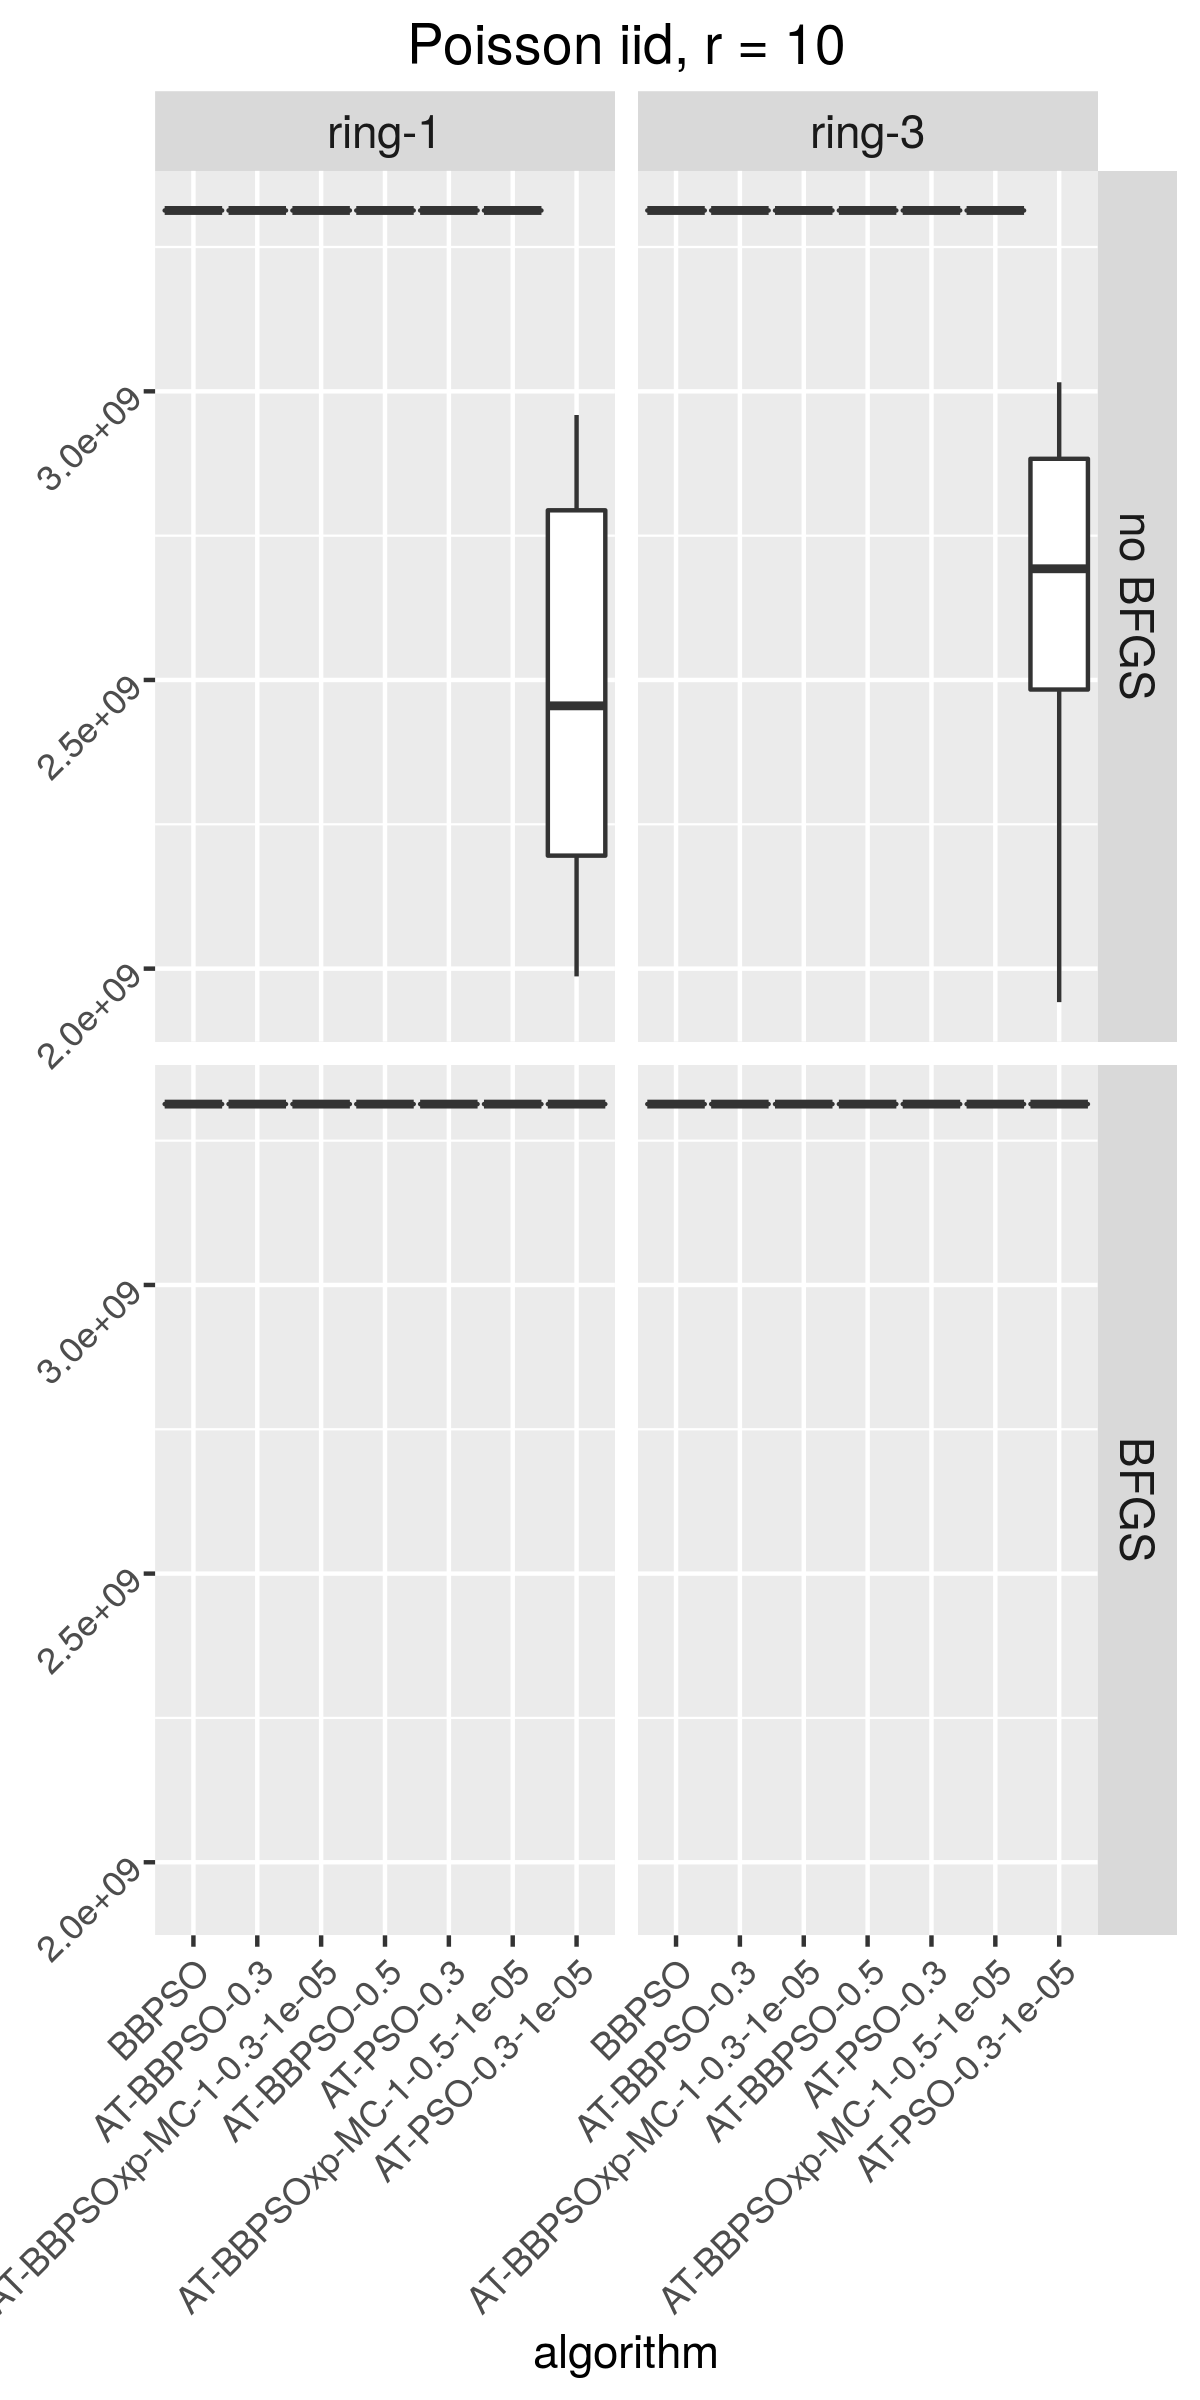
\includegraphics[width=0.4\textwidth]{code/pop/maxplot11.png}
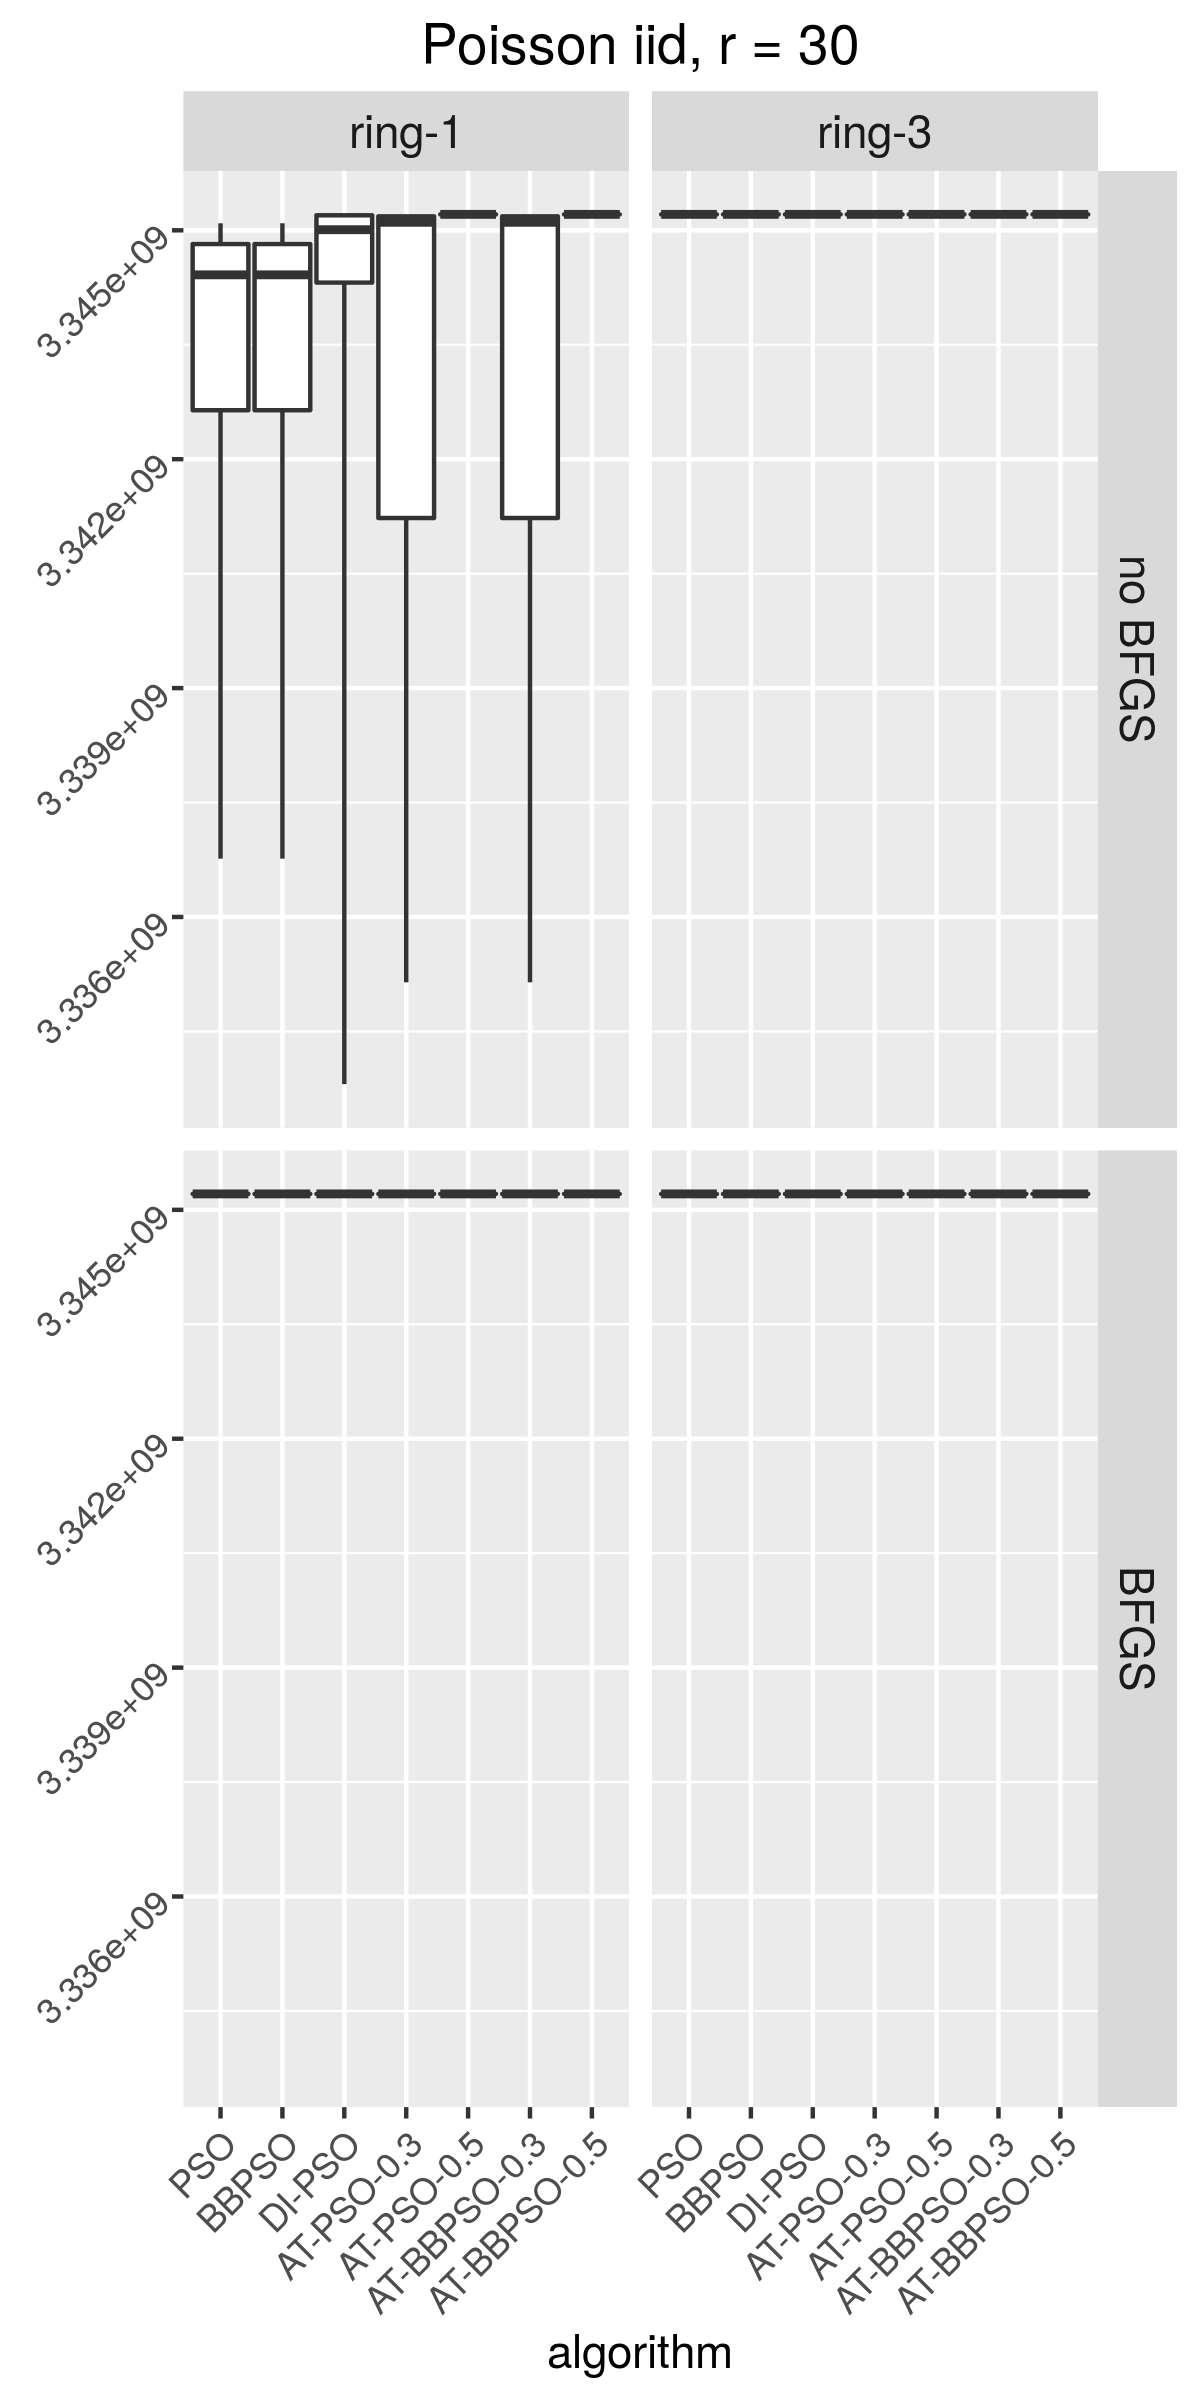
\includegraphics[width=0.4\textwidth]{code/pop/maxplot12.png}
%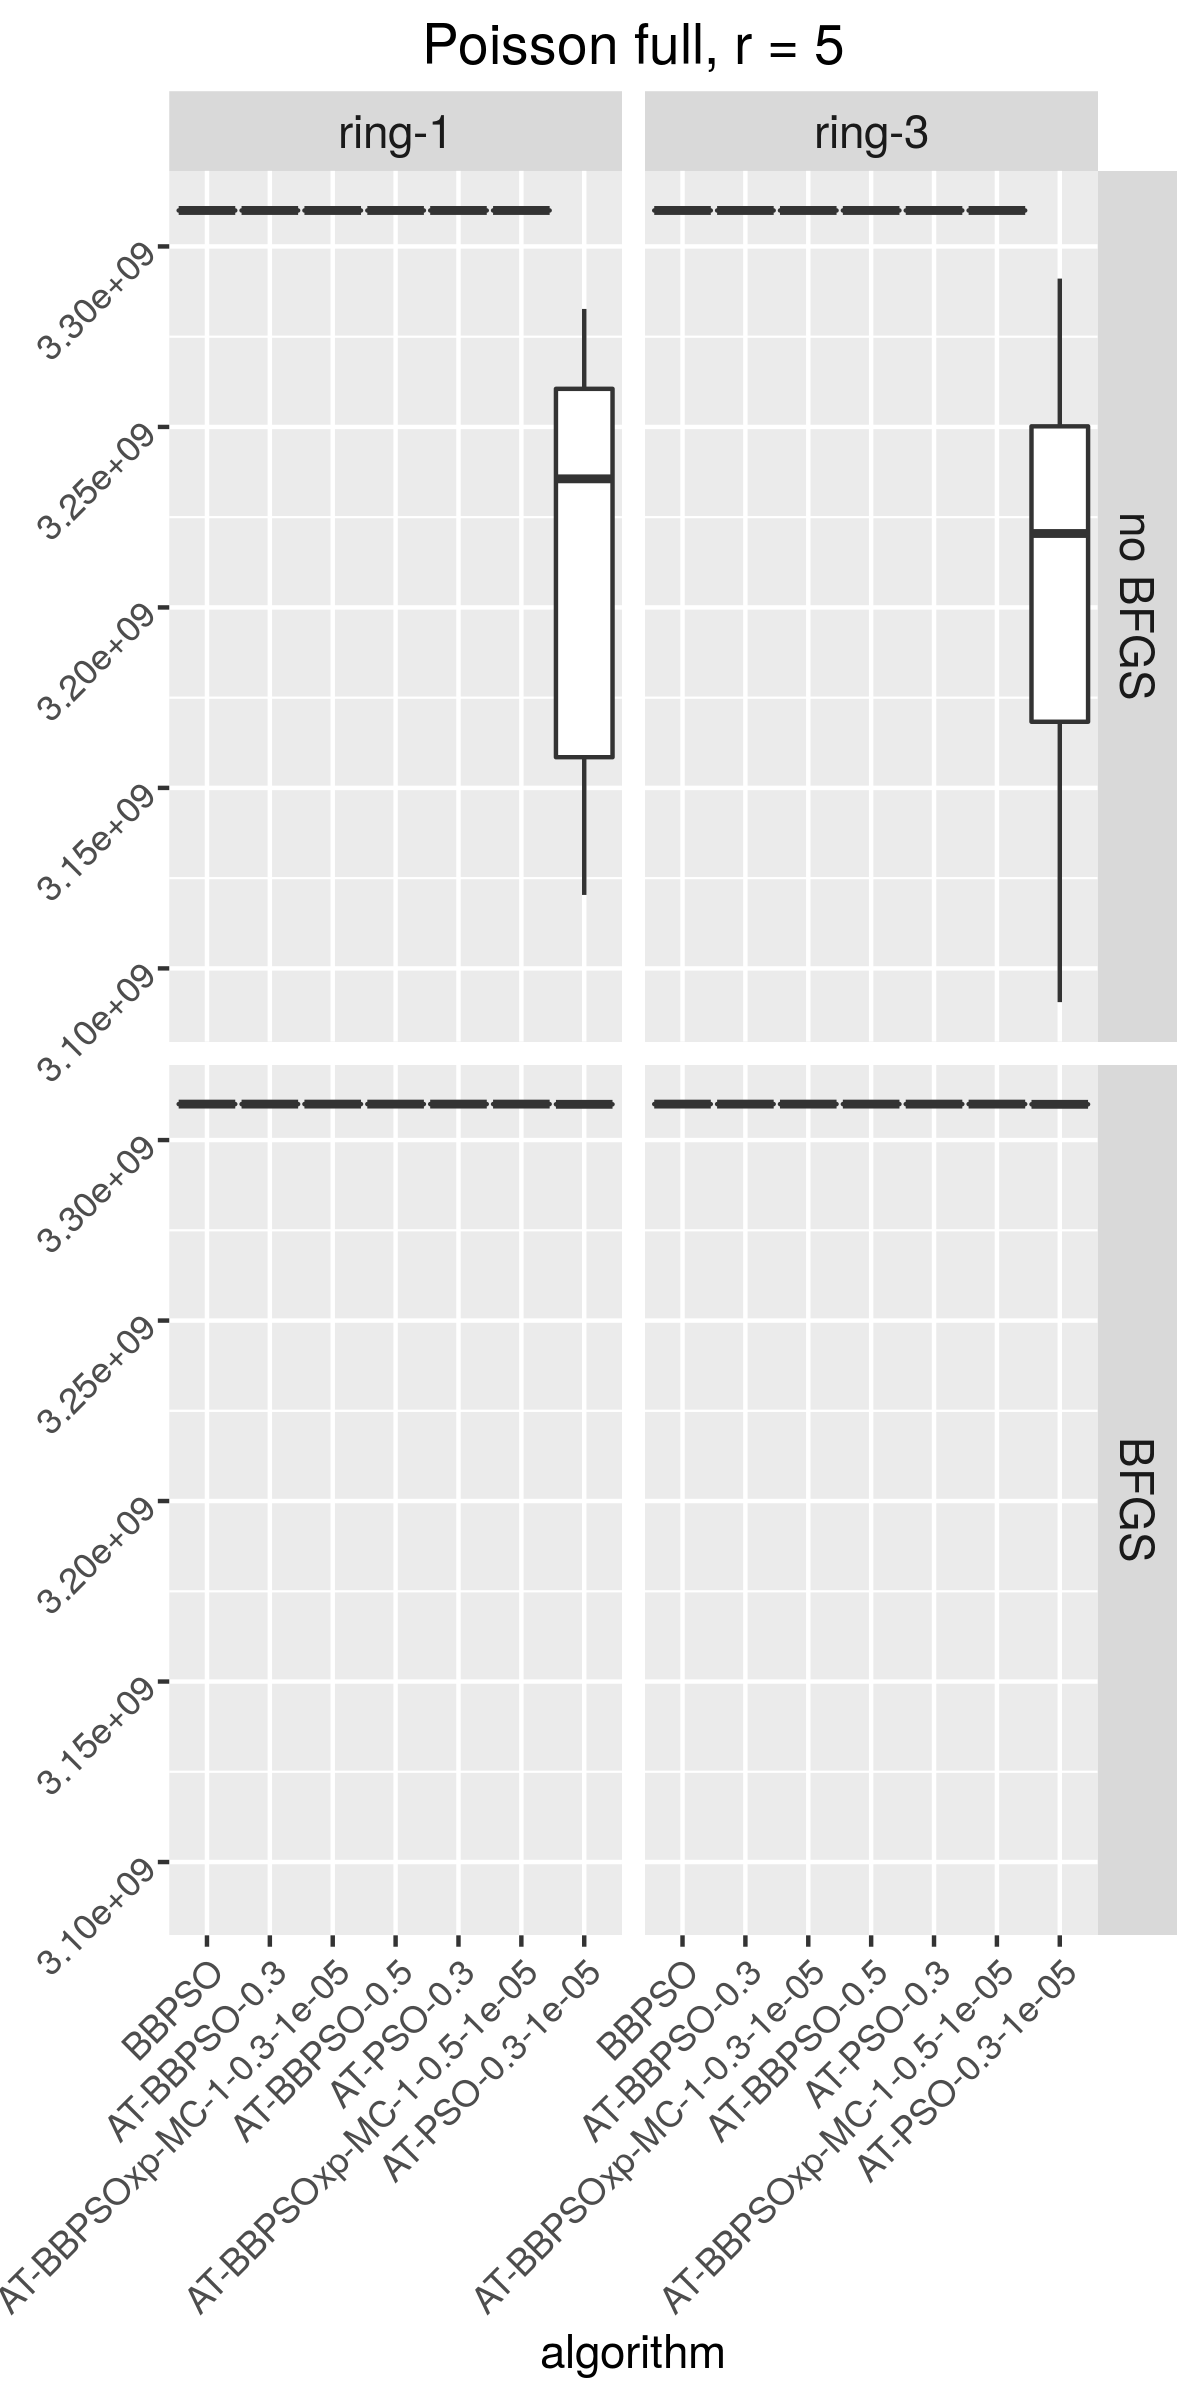
\includegraphics[width=0.4\textwidth]{code/pop/maxplot13.png}
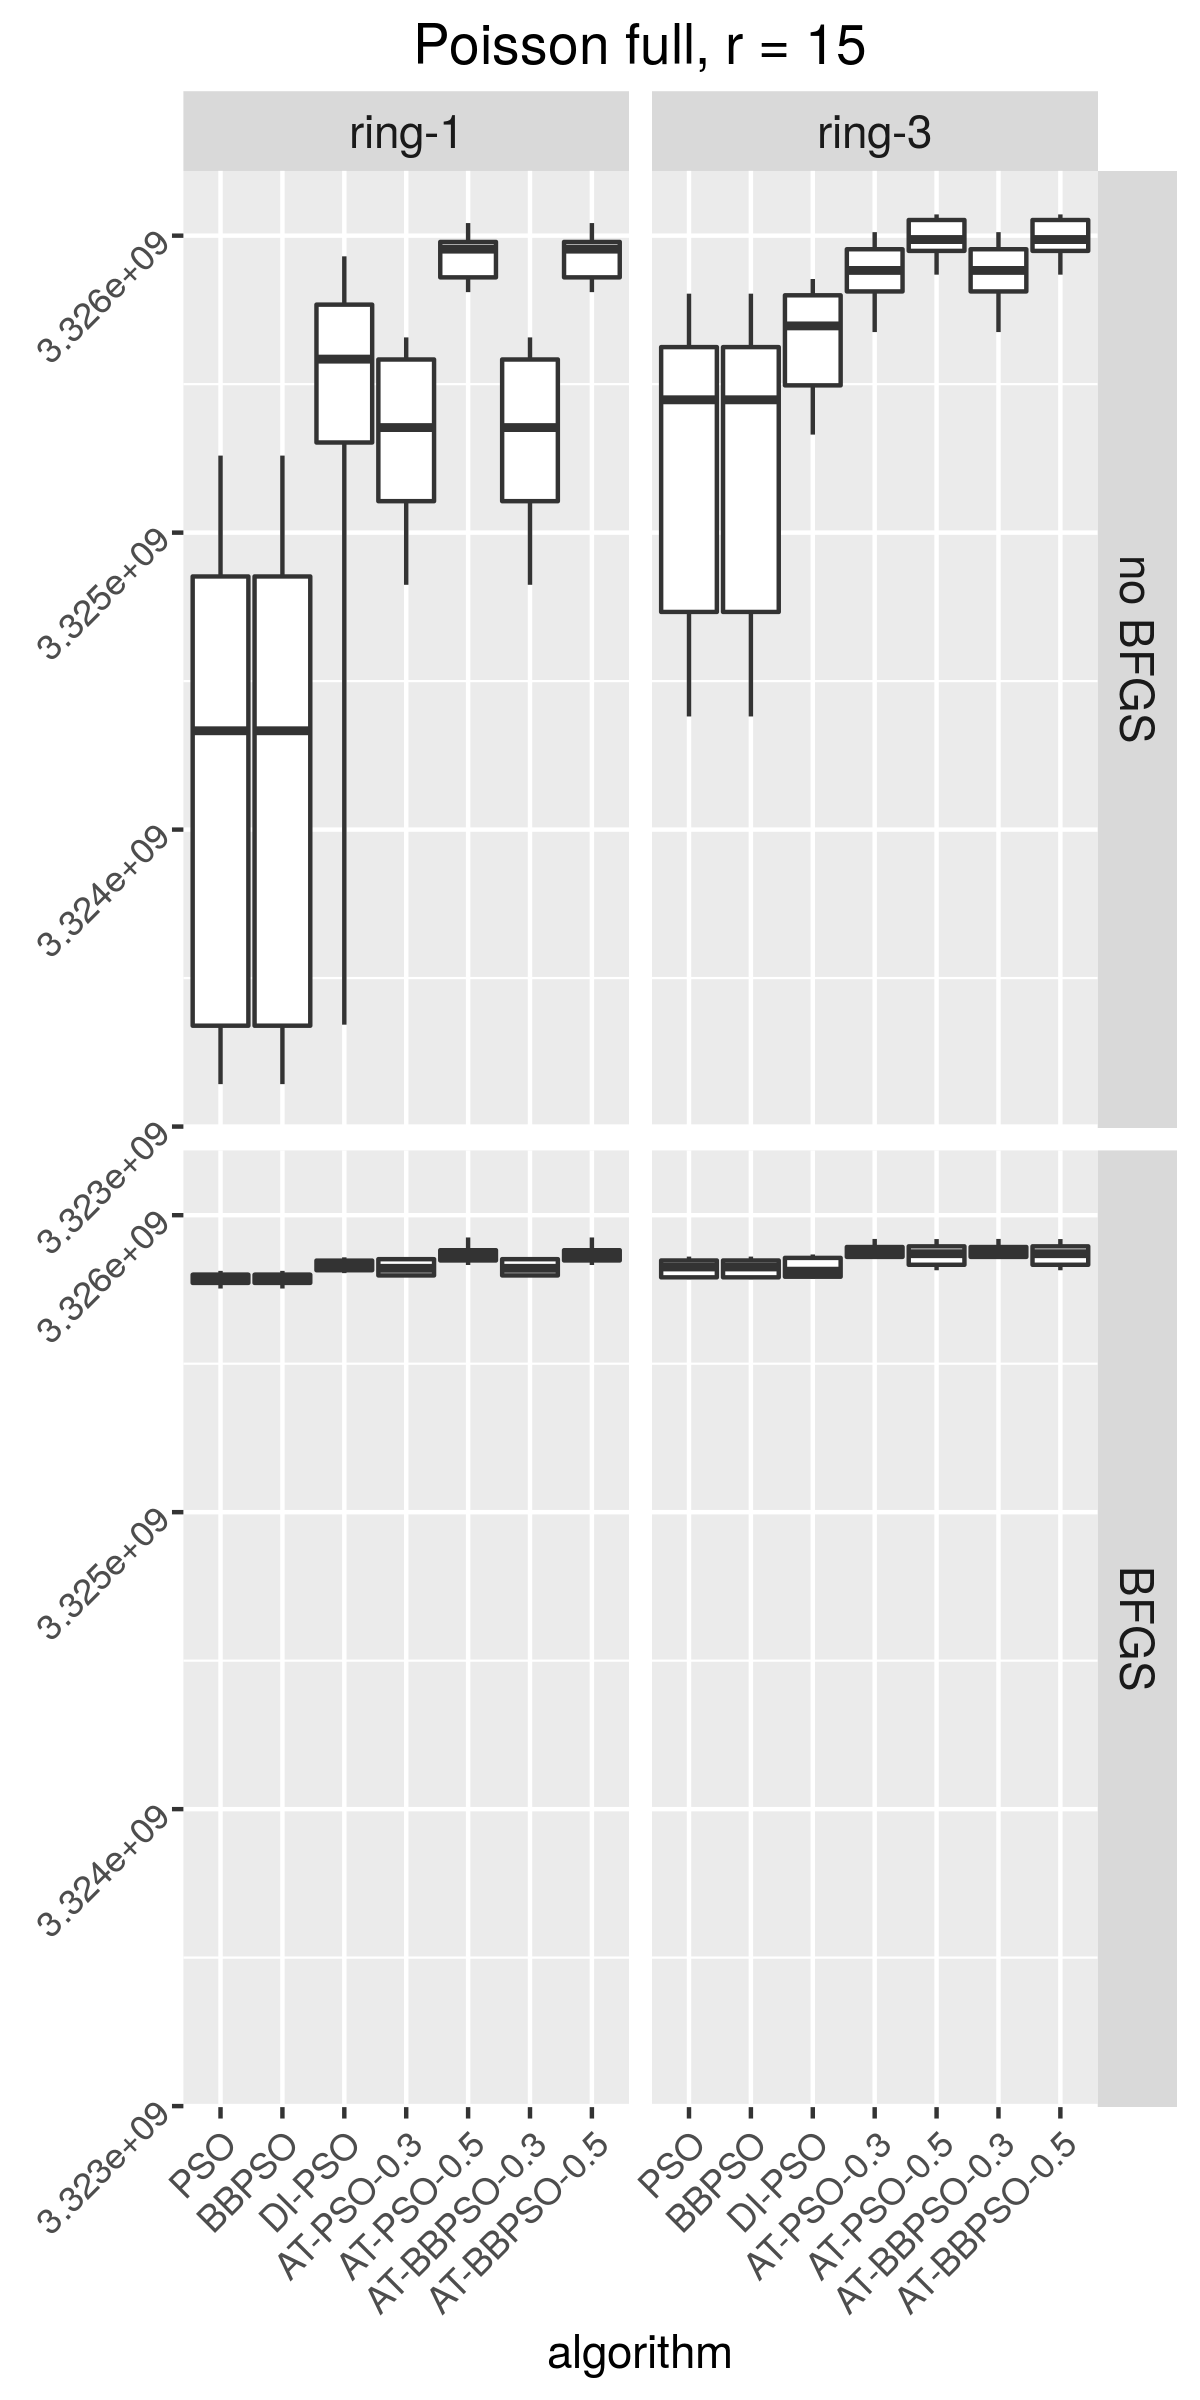
\includegraphics[width=0.4\textwidth]{code/pop/maxplot14.png}
\caption{Boxplots of the maximum value of the log posterior found for Poisson models by random effect type, neighborhood topology, optimization initialization, and algorithm. Each box plot was created using the 10, 25, 50, 75, and 90 percentiles of the maximum found from 20 replications of 1,000 iterations with 50 particles for each factor combination.}
\label{fig:popmaxboxplot}
\end{figure}

\begin{figure}[!ht]
\centering
%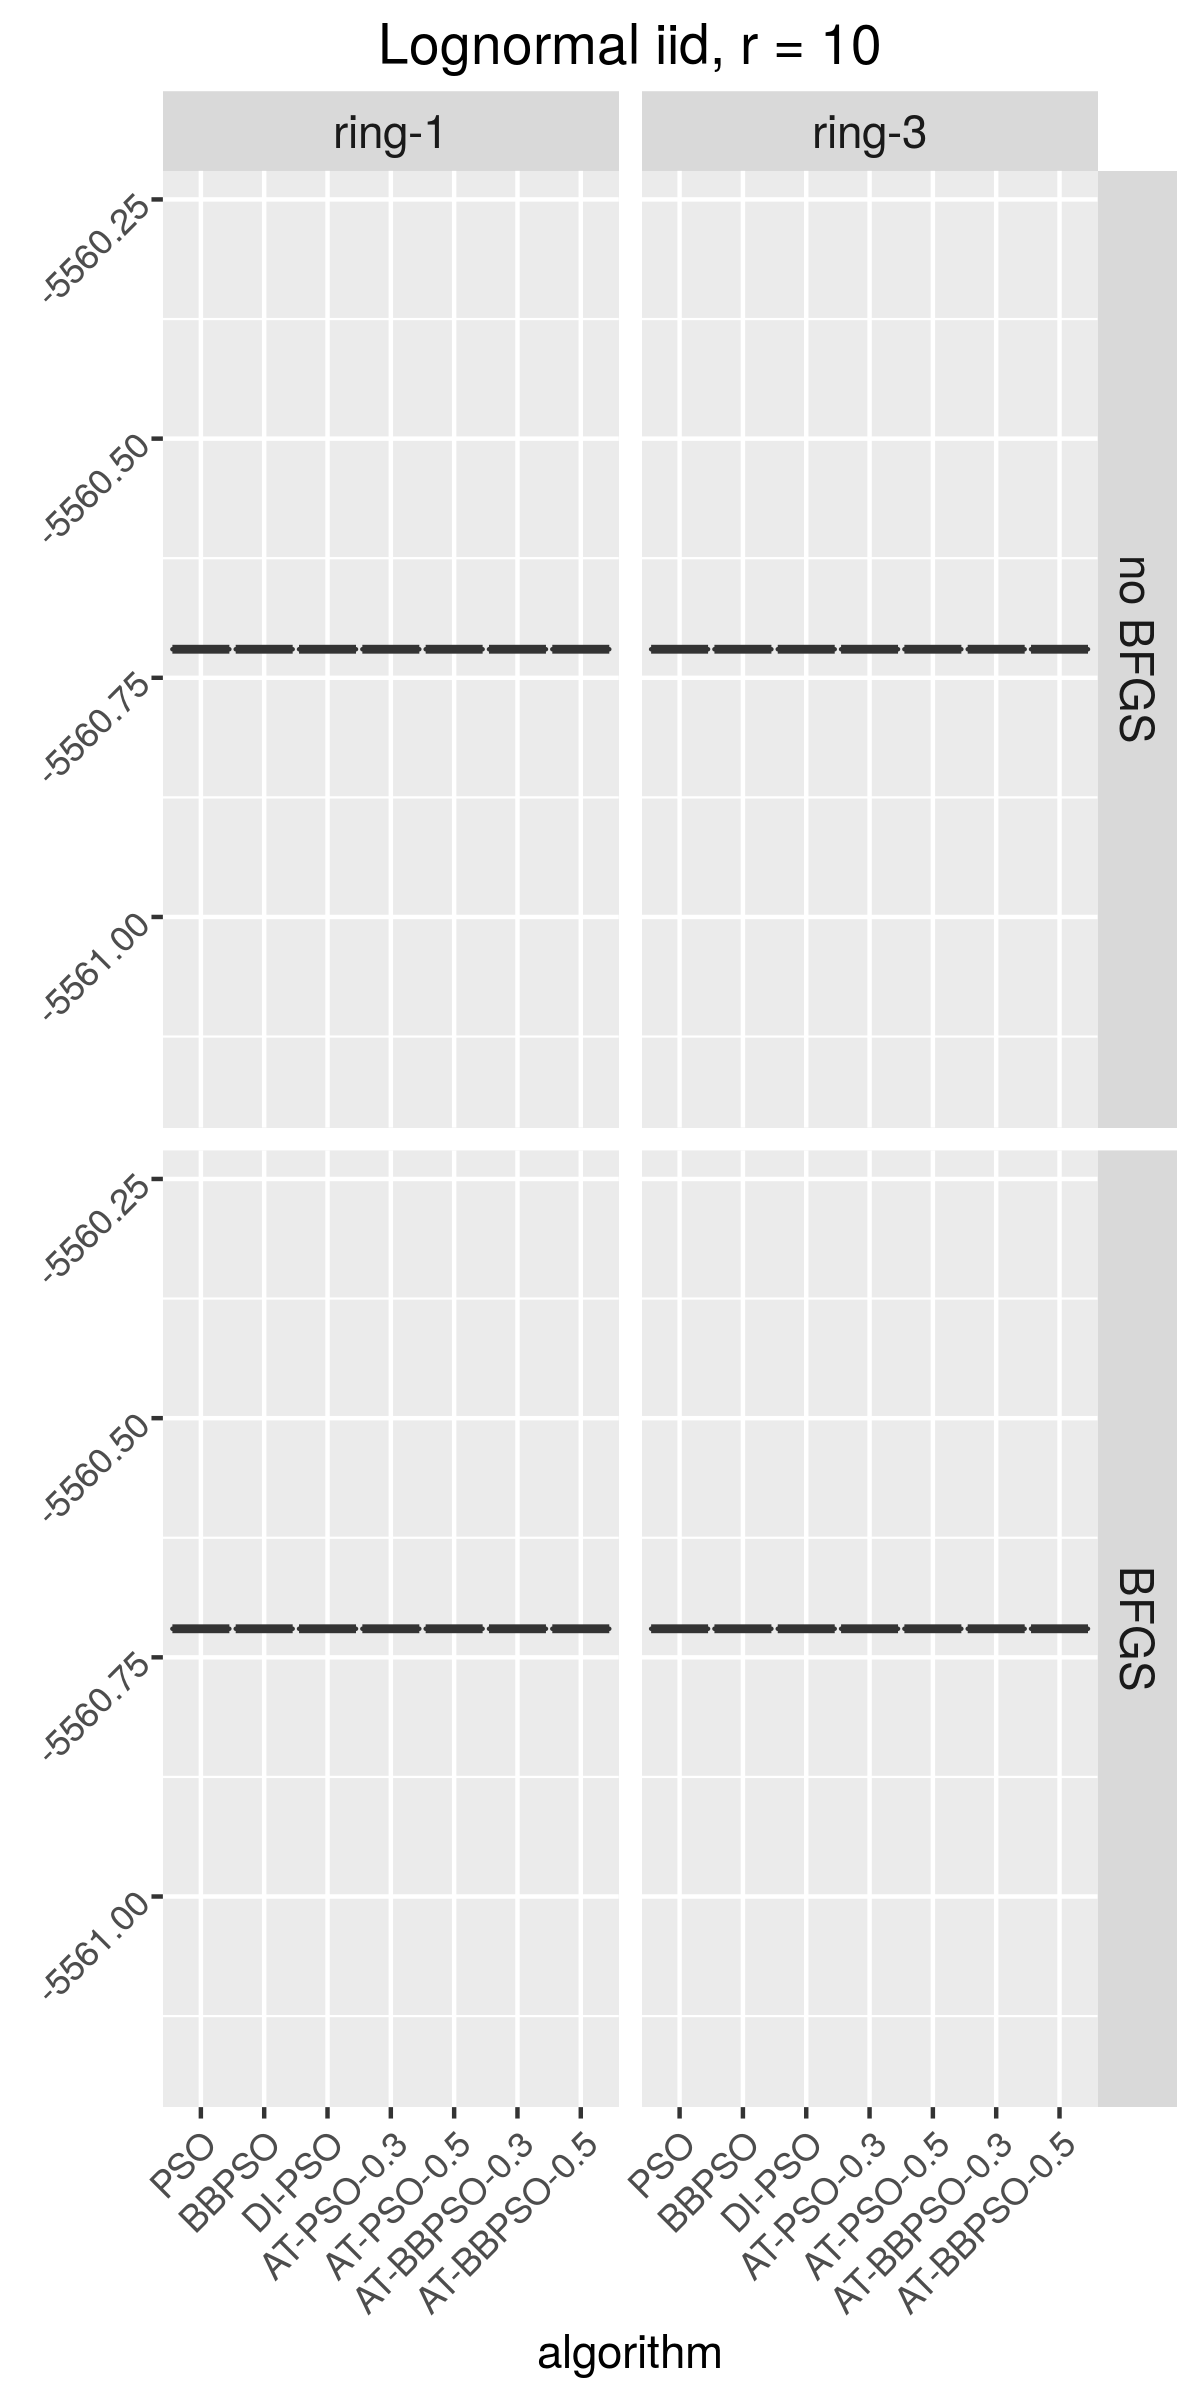
\includegraphics[width=0.4\textwidth]{code/pop/maxplot21.png}
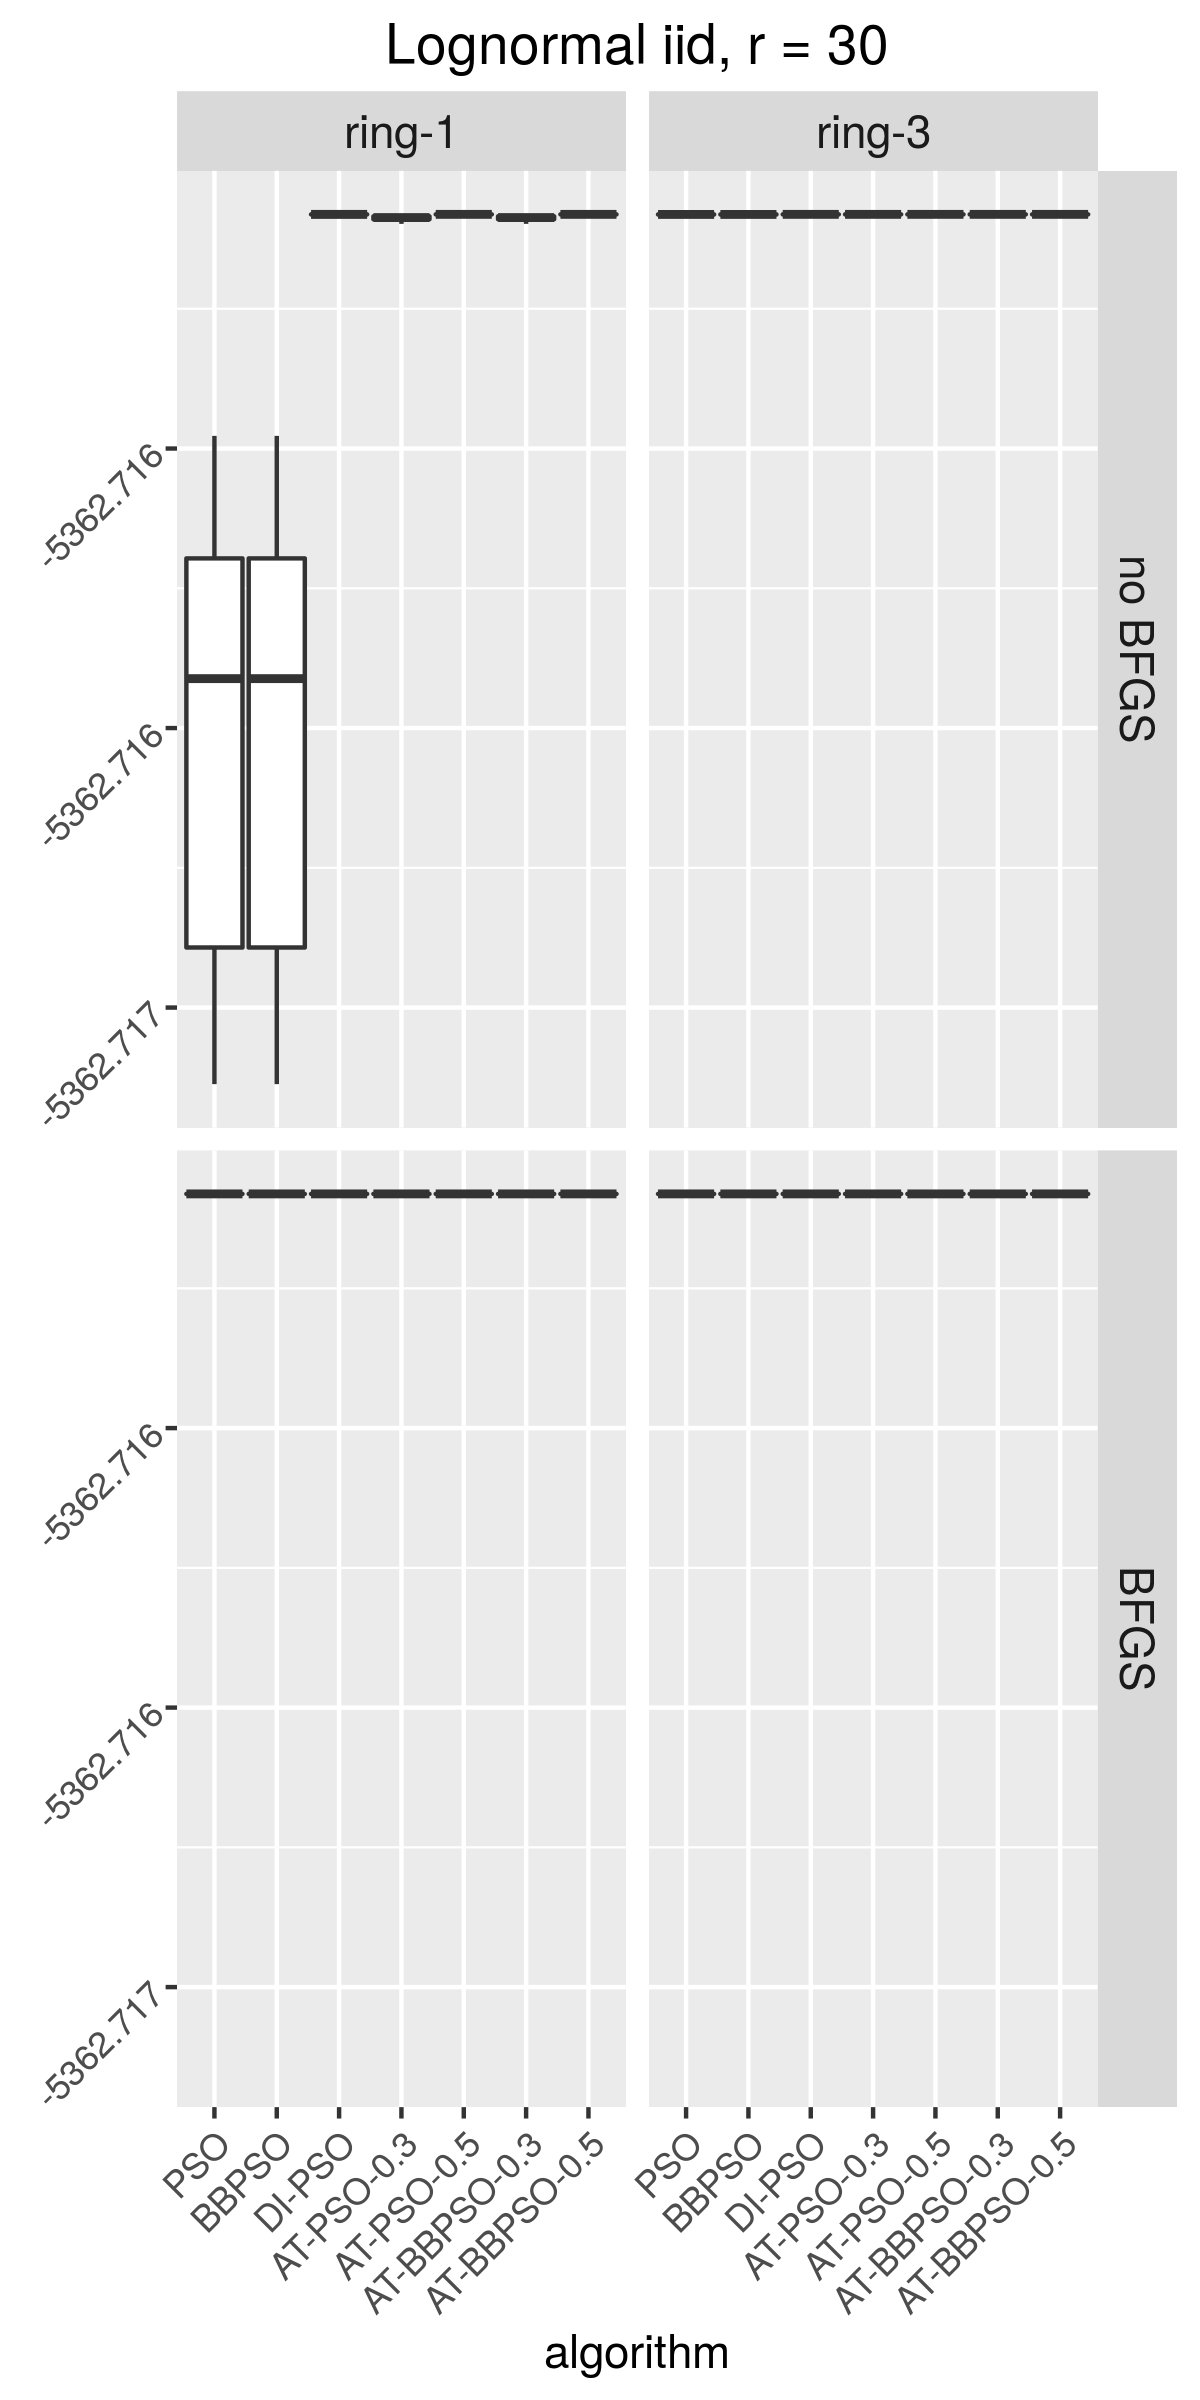
\includegraphics[width=0.4\textwidth]{code/pop/maxplot22.png}
%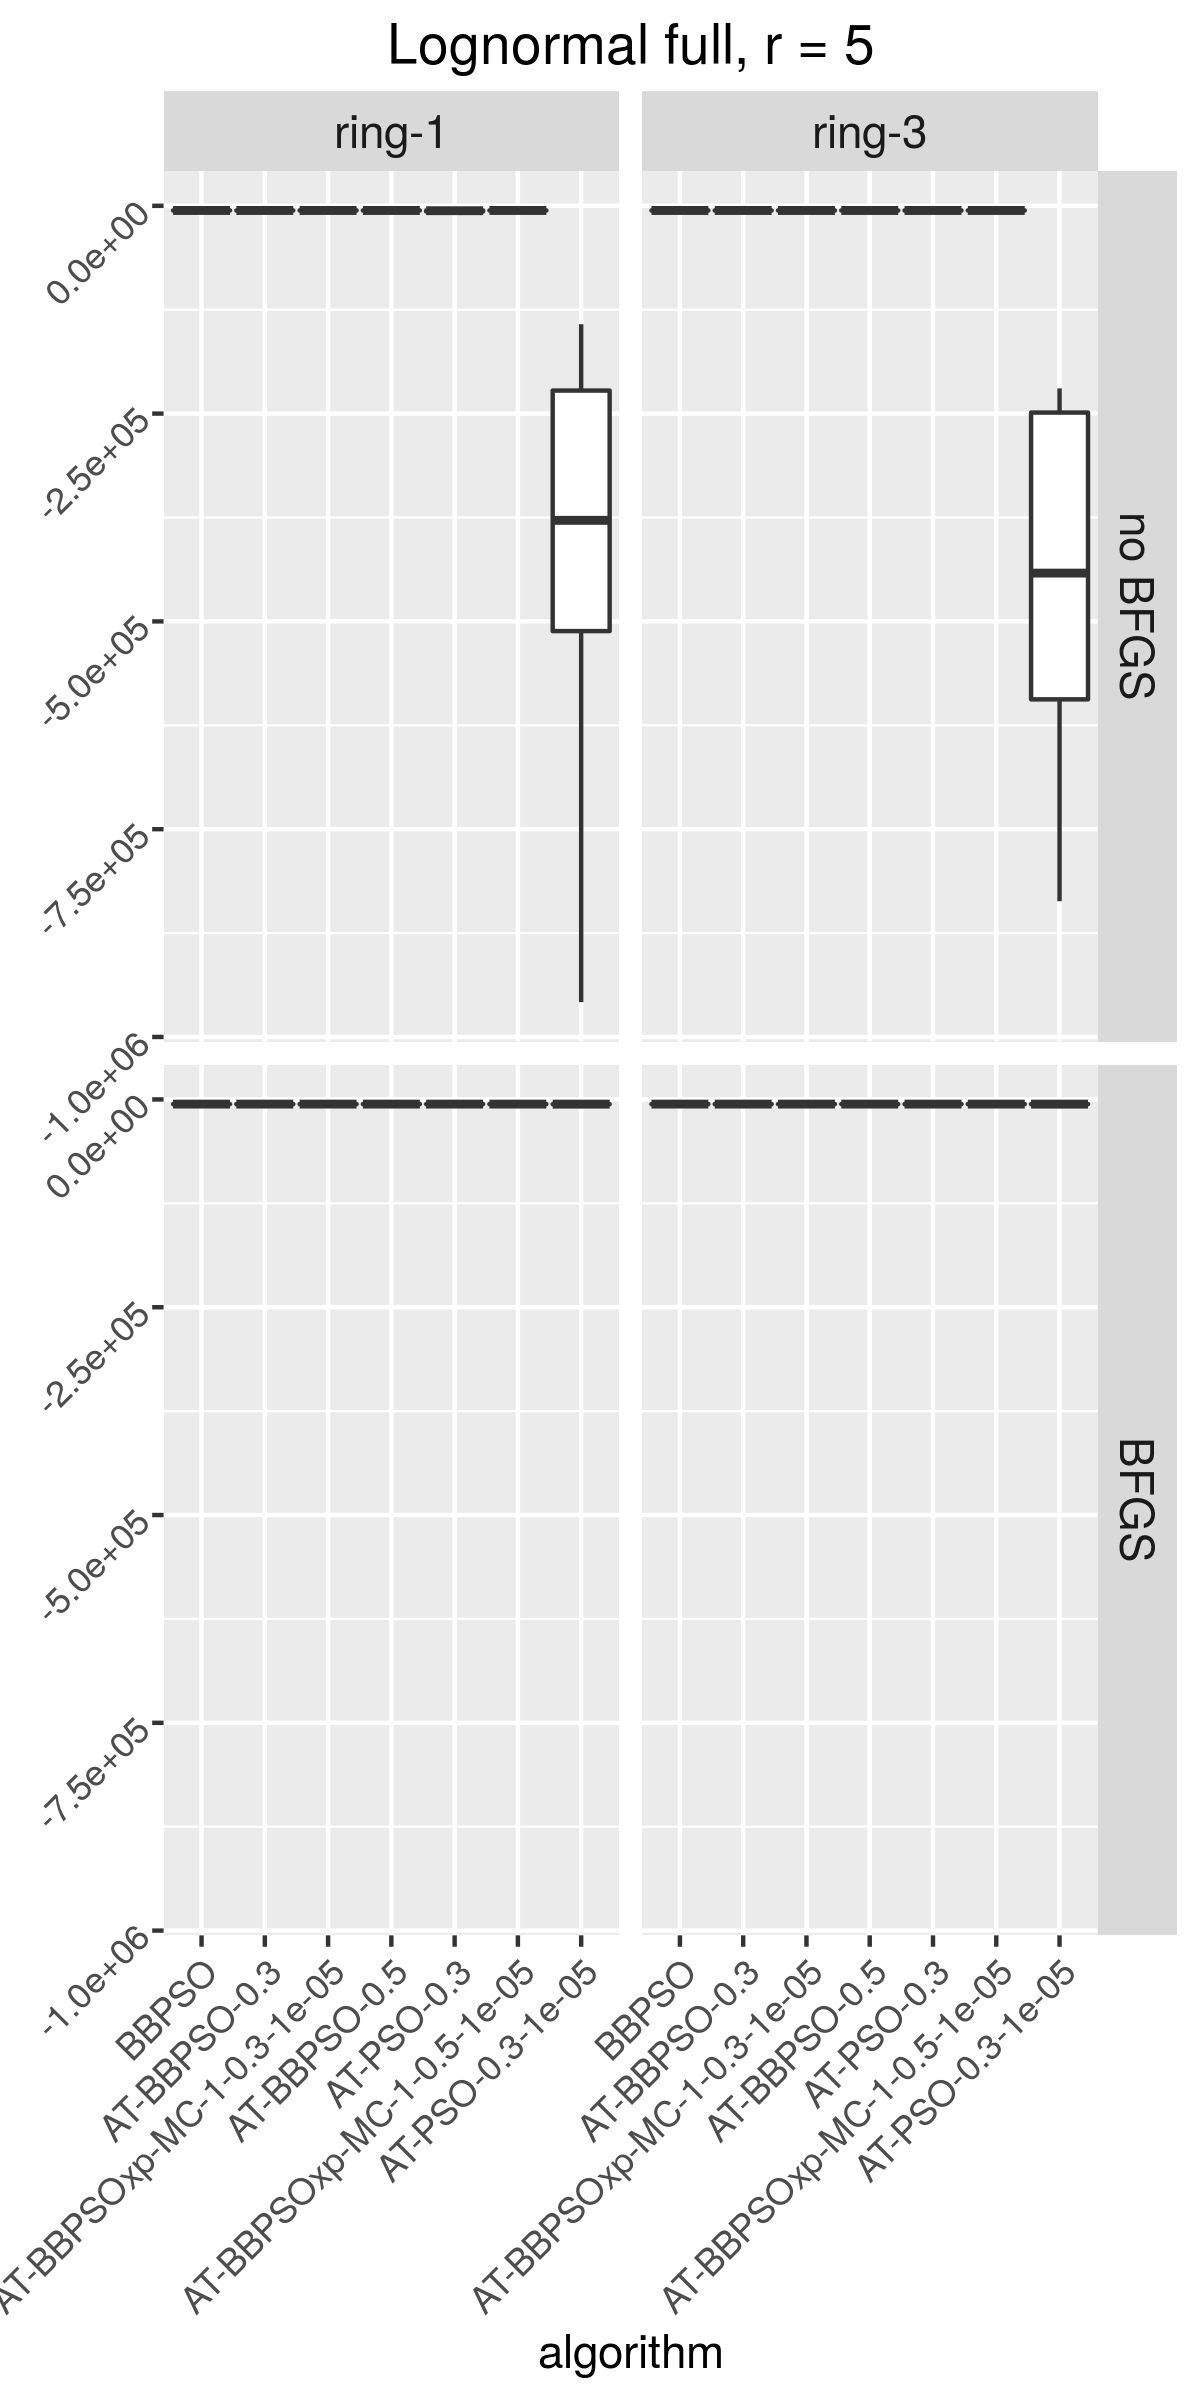
\includegraphics[width=0.4\textwidth]{code/pop/maxplot23.png}
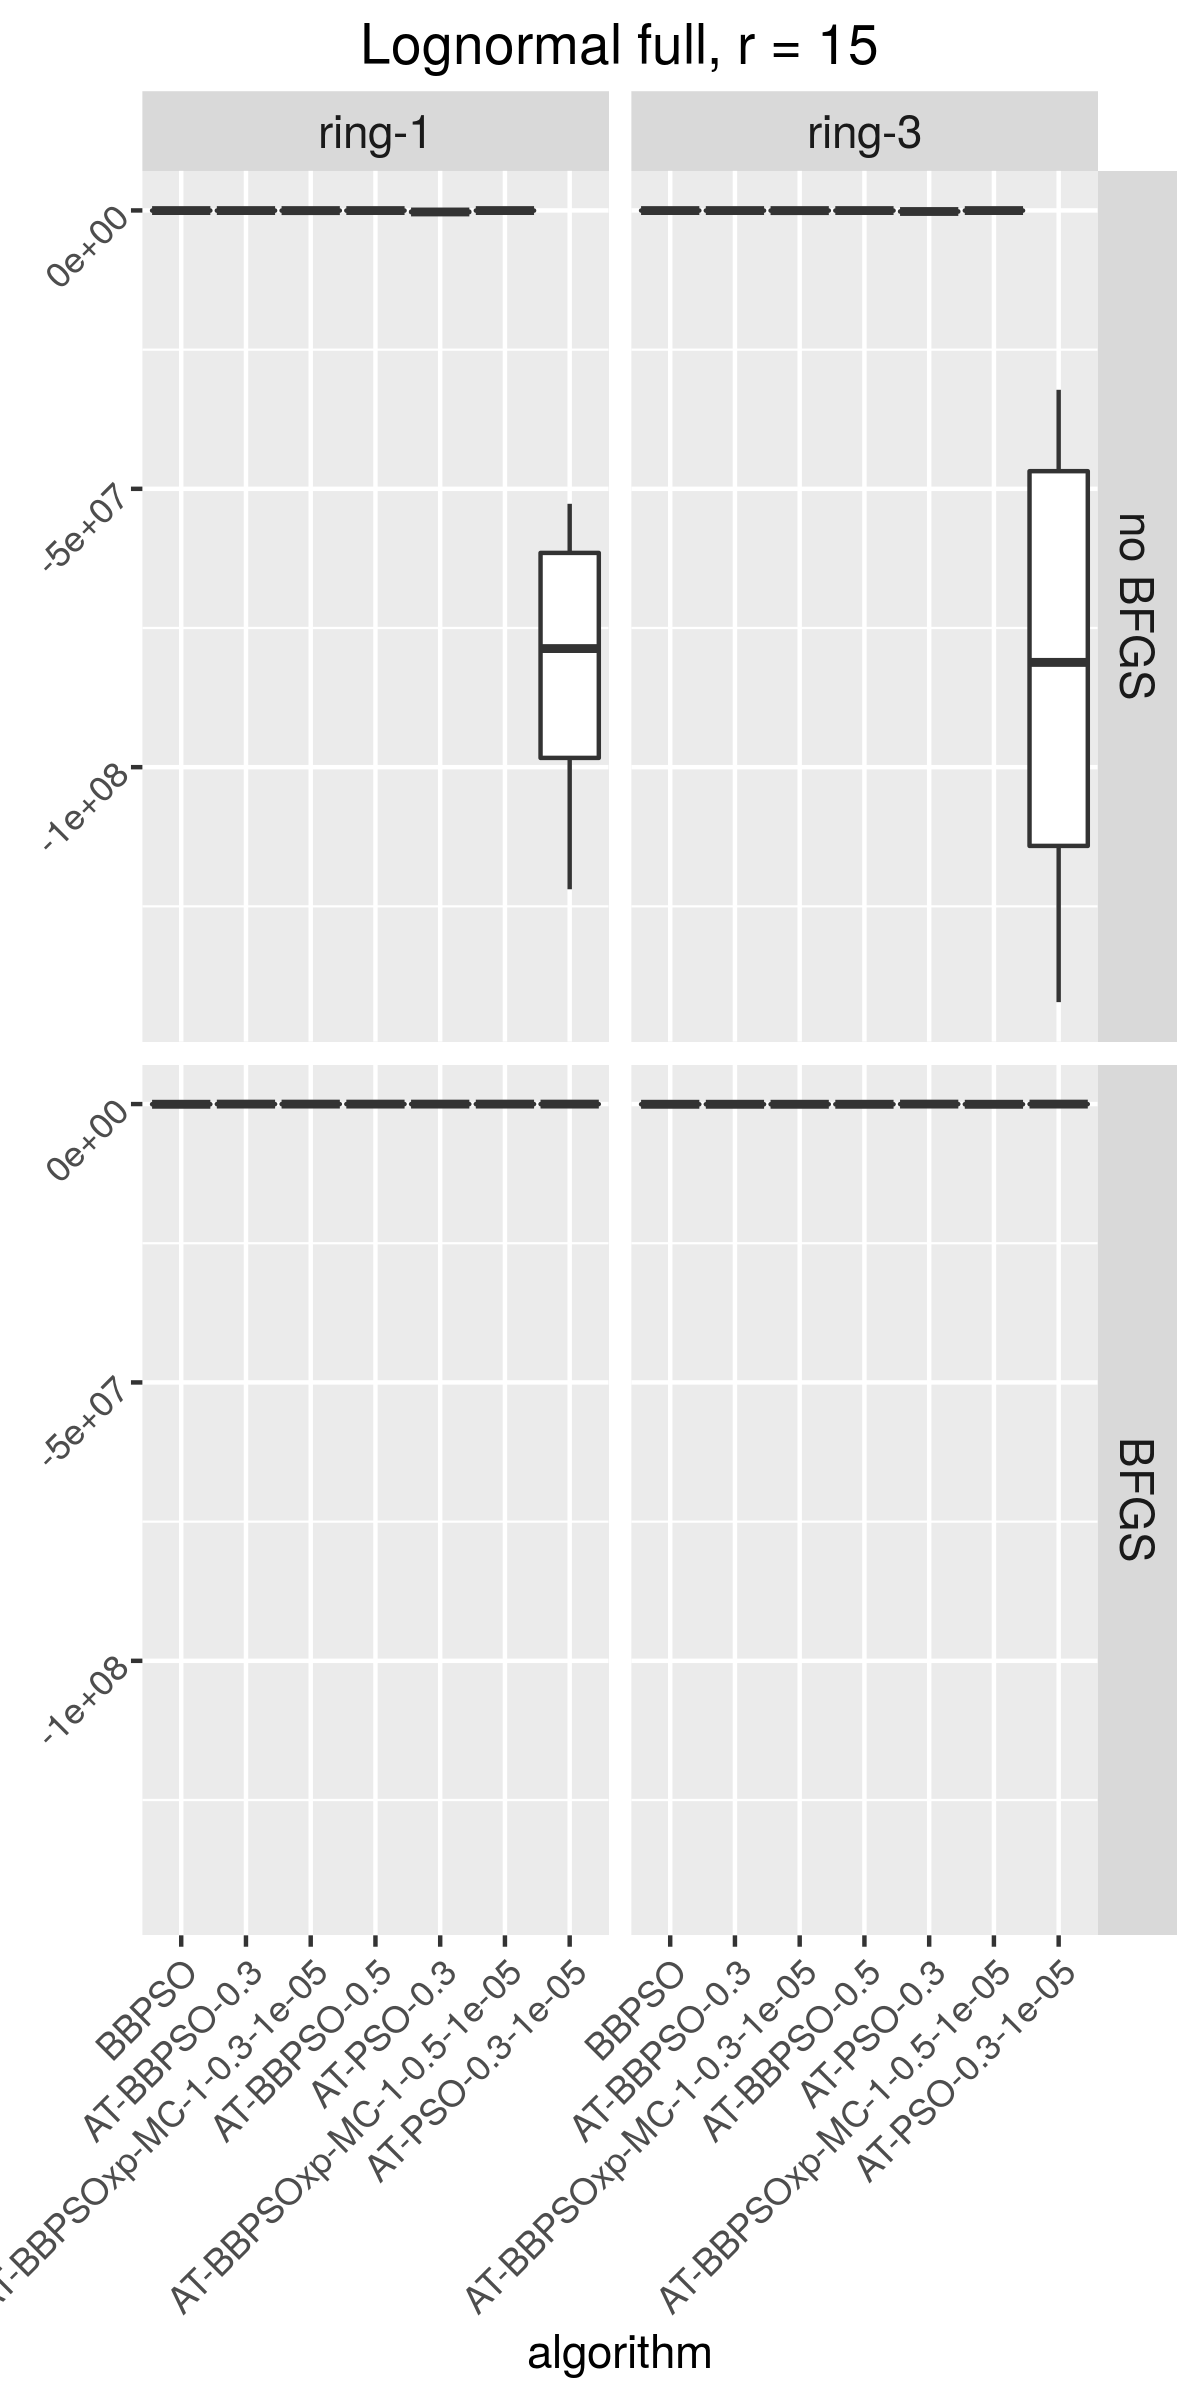
\includegraphics[width=0.4\textwidth]{code/pop/maxplot24.png}
\caption{Boxplots of the maximum value of the log posterior found for lognormal models by random effect type, number of random effects, neighborhood topology, optimization initialization, and algorithm. Each box plot was created using the 10, 25, 50, 75, and 90 percentiles of the maximum found from 20 replications of 1,000 iterations with 50 particles for each factor combination.}
\label{fig:popmaxboxplot2}
\end{figure}

[PARAGRAPH OR TWO AND PLOTS FOR THE ELECTION MODELS]

For our purposes, the PSO algorithms are useful only insofar as they allow us to construct IMH and IMHwG algorithms. So we conduct another simulation study to see when each algorithm gets close enough to the posterior mode for the IMH and IMHwG algorithms to have high acceptance rates. To this end we conduct another simulations study using the same 7 PSO algorithms from the previous study, except only using the ring-3 neighborhood topology and BFGS initialization. Next, we run the IMH and IMHwG MCMC algorithms based on 0, 100, 500, 1,000, 1,500, and 2,000 iterations of the PSO algorithm and compute the acceptance rate after 1,000 iterations of the MCMC algorithm. Each MCMC algorithm is initialized at the PSO estimate of the posterior mode used to construct the Laplace approximation. When we run the IMH and IMHwG algorithms after 0 iterations of a PSO algorithm we still run the BFGS initialization, so this serves as a control to see if running the PSO algorithm is necessary to get reasonable acceptance rates. Additionally, we run each IMH and IMHwG algorithm with different choices for the degrees of freedom parameter in the Laplace approximation.

IMH applies straightforwardly to each of our models, though see Appendix \ref{app:hess} for a detailed derivation of the Hessian for the county population models with a fully parameterized covariance matrix associated, i.e. from equations \eqref{eq:fullnormpostchol} and \eqref{eq:fullpoispostchol}. To apply IMHwG in the county population models, we draw $(\bm{\beta},\bm{\delta})$ in the Metropolis step and either $\sigma^2$ or $\bm{L}$ in the conditionally conjugate step, depending on the model. The full conditional distribution of $\sigma^2$ in \eqref{eq:iidnormpost} and \eqref{eq:iidpoispost} is $IG(a_{\sigma} + r/2, b_{\sigma} + \bm{\delta}'\bm{\delta}/2)$. The full conditional distribution of $\bm{\Omega}$ in \eqref{eq:fullnormpostprec} and \eqref{eq:fullpoispostprec} is $W(r + 1, (\bm{E} + \bm{\delta}\bm{\delta}')^{-1})$. Then a draw from the full conditional distribution of $\bm{L}$ can be obtained via the Bartlett decomposition as described at the end of Section~\ref{sec:pop}. In the lognormal models the full conditional distribution of $\phi^2$ is $IG(a_{\phi} + n/2, b_{\phi} + (\log \bm{z} - \bm{X}\bm{\beta} - \bm{S}\bm{\delta})'(\log \bm{z} - \bm{X}\bm{\beta} - \bm{S}\bm{\delta})/2)$. 

In single poll model of Section~\ref{sec:pres}, we draw $(\beta_0, \beta_f, \beta_b, \bm{\alpha}_{s}, \bm{\alpha}_{ae})$ in the Metropolis step, while in the all polls model we draw all of those parameters and additionally $\bm{\alpha}_p$ in the Metropolis step. Then for both models there are two additional Gibbs steps --- one where each random effect variance is drawn, and one where $(\beta_{prev}, \bm{\alpha}_r)$ is drawn. These full conditionals are straightforward to derive, so we do not reproduce them here. Likewise, the Hessian is easy though tedious to derive, so we omit it as well.

[SIMULATION STUDY TO BE COMPLETED AND PUT HERE - WON'T TAKE VERY LONG, ~ 1 DAY]

% In their conditional posterior, the random effects variances are independent with
% \begin{align*}
% \sigma^2_{s} &\sim IG\left(a_{s} + 51/2, b_{s} + \sum_{k=1}^{51}(\alpha_{s}[k] - \alpha_r[r_k] - prev_k\beta_{prev})^2/2\right)\\
% \sigma^2_{ae} &\sim IG(a_{ae} + 16/2, b_{ae} + \bm{\alpha}_{ae}'\bm{\alpha}_{ae}/2)\\
% \sigma^2_{p} &\sim IG(a_{p} + 7/2, b_{p} + \bm{\alpha}_{p}'\bm{\alpha}_{p}/2)\\
% \sigma^2_{r} &\sim IG(a_{r} + 5/2, b_{r} + \bm{\alpha}_{r}'\bm{\alpha}_{r}/2)
% \end{align*}
% where in the prior we set $a_{s}=a_{ae}=a_p=a_r=b_{s}=b_{ae}=b_p=b_r=1$. These full conditionals apply to both the single poll and all polls models, except $\sigma_p^2$ is not included

% First we consider the acceptance rates of the PSO assisted IMH and IMHwG algorithms. Table \ref{tab:accrates} contains computed acceptance rates for each of the PSO assisted algorithms and for each model for spatially smoothing county population estimates. For each model we used the default PSO algorithm to find the posterior mode with a swarm of 50 particles run for 1000 iterations using the ring-1 neighborhood. For any given model and choice of $df$ the IMH within Gibbs algorithm tends to have a higher acceptance rate --- indeed for the full Poisson model with $r=5$ or $r=7$, only the IMH winin Gibbs algorithms yields acceptable acceptance rates. The $t$ proposal also tends to do better with higher $df$ indicating that tails of the posterior are approximately normal --- indeed a $t$ distribution with $df=100$ is nearly identical to a normal distribution. Also notable is that acceptance rates for the lognormal model tend to be higher than for the Poisson model, illustrating that the closer the data model is to Gaussian the better the IMH and IMHwG algorithms based on the Laplace approximation are going to perform.

% \begin{table}[ht]
% \captionsetup{font=footnotesize}
% \centering
% \subfloat[PSO assisted independent Metropolis Hastings acceptance rates]{
% \footnotesize{
% \begin{tabular}{r|rrr|rrr|rrr|rrr}
% \multicolumn{1}{c}{IMH\phantom{wG}} & \multicolumn{3}{c}{iid lognormal}&\multicolumn{3}{c}{iid Poisson} & \multicolumn{3}{c}{full lognormal}&\multicolumn{3}{c}{full Poisson}\\
%   \hline
% df & r = 10 & 20 & 30 & 10 & 20 & 30 & 5 & 7 & 9 & 5 & 7 & 9 \\  
%   \hline
% 1 & 0.24 & 0.19 & 0.15 & 0.29 & 0.23 & 0.09 & 0.00 & 0.00 & 0.00 & 0.01 & 0.00 & 0.01 \\ 
%   4 & 0.47 & 0.37 & 0.32 & 0.54 & 0.45 & 0.18 & 0.01 & 0.00 & 0.00 & 0.01 & 0.00 & 0.00 \\ 
%   10 & 0.60 & 0.52 & 0.46 & 0.71 & 0.63 & 0.25 & 0.02 & 0.00 & 0.00 & 0.03 & 0.00 & 0.00 \\ 
%   100 & 0.72 & 0.70 & 0.68 & 0.88 & 0.88 & 0.37 & 0.02 & 0.00 & 0.00 & 0.03 & 0.01 & 0.00 \\ 
%    \hline
% \end{tabular}}}\\
% %\vspace*{0.5 cm}
% \subfloat[PSO assisted independent Metropolis Hastings within Gibbs acceptance rates]{
% \footnotesize{
% \begin{tabular}{r|rrr|rrr|rrr|rrr}
% \multicolumn{1}{c}{IMHwG} & \multicolumn{3}{c}{iid lognormal}&\multicolumn{3}{c}{iid Poisson} & \multicolumn{3}{c}{full lognormal}&\multicolumn{3}{c}{full Poisson}\\
%   \hline
% df & r = 10 & 20 & 30 & 10 & 20 & 30 & 5 & 7 & 9 & 5 & 7 & 9 \\  
%   \hline
% 1 & 0.31 & 0.23 & 0.19 & 0.31 & 0.23 & 0.11 & 0.01 & 0.00 & 0.00 & 0.17 & 0.17 & 0.06 \\ 
%   4 & 0.58 & 0.46 & 0.40 & 0.58 & 0.46 & 0.18 & 0.01 & 0.00 & 0.00 & 0.57 & 0.12 & 0.07 \\ 
%   10 & 0.75 & 0.65 & 0.56 & 0.76 & 0.64 & 0.27 & 0.01 & 0.00 & 0.00 & 0.44 & 0.11 & 0.09 \\ 
%   100 & 0.94 & 0.92 & 0.89 & 0.96 & 0.94 & 0.36 & 0.02 & 0.00 & 0.00 & 0.50 & 0.14 & 0.03 \\ 
%    \hline
% \end{tabular}}}
% \caption{ Acceptance rates for the PSO assisted IMH algorithm (a) and the IMH within Gibbs algorithm (b) in the Poisson and lognormal models with either iid or fully correlated random effects. For each algorithm and each model the initial posterior mode was estimated using the default PSO algorithm, then acceptance rates were computed from a sample of 9000 after a burn-in of 1000. The parameter $r$ denotes the number of random effects in the model and $df$ denotes the degrees of freedom parameter used in the $t$ proposal.}
% \label{tab:accrates}
% \end{table}

% Both the full Poisson and full lognormal model cause problems because the fully parameterized covariance matrix means that the normal approximation will be poor for those parameters. In the iid case the random effect variance essentially has $r$ observations --- one for each random effect --- but in the full model we have an $r\times r$ covariance matrix with essentially one observation ($\bm{\delta}$). The Laplace approximation is an asymptotic result so with such a small amount of data it is no surprise that it is poor. However, IMHwG still works well for the Poisson model when the dimension of $\bm{\delta}$ is small enough --- in this case $r=5$. The conditional posterior of $(\bm{\beta}, \bm{\delta})$ given $\bm{L}$ should approximated well by a $t$ distribution even for larger $r$ given the amount of observed data and the normal priors on $\bm{\beta}$ and $\bm{\delta}$. The problem is that our estimate of the mode is poor, though this can be solved with enough patience.

% While Table \ref{tab:accrates} used the same PSO algorithm to investigate acceptance rates, Table \ref{tab:longaccrates} uses a variety of different PSO algorithms. Four algorithms are considered: standard PSO, BBPSOxp-MC, AT-BBPSOxp-MC with $df=1$ and $R^*=0.1$, and AT-BBPSOxp-MC with $df=5$ and $R^*=0.3$. Each algorith was run with 1,000 particles in a ring-1 neighborhood for 10,000 iterations. Finally, the IMH and IMHwG MCMC algorithms were run multiple times for each PSO algorithm, using the PSO algorithm's estimate of the mode after 100, 1,000, 5,000, and 10,000 iterations. A key takeaway from Table \ref{tab:longaccrates} is that in many conditions the main reason that IMH and IMHwG have poor acceptance rates is that the PSO algorithm has failed to adequately estimate the posterior mode. In Table \ref{tab:accrates}, both algorithms had trouble with the fully parameterized Poisson model. But using a larger swarm size and many more iterations, the standard PSO algorithm yields IMH algorithms with low but acceptable acceptance rates and IMHwG algrithms with near 100\% acceptance rates --- at least for $r=5$ and $r=10$. For $r=15$ the MCMC algorithm fails, but examination of Figure \ref{fig:longpsopoisfull15} shows that the PSO algorithm has not converged even after 10,000 iterations. Running the algorithm longer or using the same amount of iterations with a larger swarm size could result in convergence and, as a result, yield better Metropolis acceptance rates at the cost of more time spent on computation. The upshot is that at least for the Poisson model using this data, the IMHwG algorithm seems to always have near 100\% acceptance rates if you can find the posterior mode. As the dimension of the optimization problem grows, however, this becomes an increasingly costly problem to solve.

% \begin{table}[ht]
% \captionsetup{font=footnotesize}
% \centering
% \subfloat[PSO assisted independent Metropolis Hastings acceptance rates]{
% \footnotesize{
% \begin{tabular}{l|r|rrr|rrr|rrr|rrr}
% \multicolumn{2}{l}{IMH} & \multicolumn{3}{c}{iid lognormal} & \multicolumn{3}{c}{iid Poisson} & \multicolumn{3}{c}{full lognormal} & \multicolumn{3}{c}{full Poisson} \\
%   \hline
% \multicolumn{1}{c|}{PSO alg} & \multicolumn{1}{c|}{$n_{\text{iter}}$} & r = 10 & 30 & 50 & 10 & 30 & 50 & 5 & 10 & 15 & 5 & 10 & 15\\
%   \hline
% PSO & 100 & 0.21 & 0.02 & 0.01 & 0.00 & 0.43 & 0.50 & 0.01 & 0.00 & 0.00 & 0.04 & 0.10 & 0.18 \\ 
% BBPSOxp-MC&  & 0.59 & 0.02 & 0.00 & 0.31 & 0.12 & 0.24 & 0.01 & 0.00 & 0.00 & 0.02 & 0.03 & 0.04 \\ 
% AT-1-0.1 &  & 0.67 & 0.00 & 0.00 & 0.23 & 0.00 & 0.30 & 0.00 & 0.00 & 0.00 & 0.01 & 0.03 & 0.05 \\ 
% AT-5-0.3 &  & 0.55 & 0.01 & 0.00 & 0.31 & 0.12 & 0.27 & 0.01 & 0.00 & 0.00 & 0.03 & 0.03 & 0.06 \\ 
% \hline
% PSO & 1,000 & 0.71 & 0.67 & 0.58 & 0.89 & 0.25 & 0.01 & 0.01 & 0.00 & 0.00 & 0.27 & 0.01 & 0.04 \\ 
% BBPSOxp-MC&  & 0.71 & 0.66 & 0.51 & 0.88 & 0.01 & 0.02 & 0.01 & 0.00 & 0.00 & 0.02 & 0.00 & 0.01 \\ 
% AT-1-0.1 &  & 0.72 & 0.66 & 0.53 & 0.88 & 0.01 & 0.02 & 0.01 & 0.00 & 0.00 & 0.04 & 0.01 & 0.01 \\ 
% AT-5-0.3 &  & 0.71 & 0.65 & 0.54 & 0.88 & 0.02 & 0.02 & 0.01 & 0.00 & 0.00 & 0.05 & 0.00 & 0.01 \\ 
% \hline
% PSO & 5,000 & 0.70 & 0.66 & 0.54 & 0.89 & 0.88 & 0.85 & 0.03 & 0.00 & 0.00 & 0.00 & 0.05 & 0.02 \\ 
% BBPSOxp-MC&  & 0.73 & 0.64 & 0.54 & 0.89 & 0.01 & 0.01 & 0.00 & 0.00 & 0.00 & 0.20 & 0.00 & 0.01 \\ 
% AT-1-0.1 &  & 0.72 & 0.68 & 0.58 & 0.89 & 0.10 & 0.00 & 0.04 & 0.00 & 0.00 & 0.37 & 0.00 & 0.01 \\ 
% AT-5-0.3 &  & 0.71 & 0.67 & 0.55 & 0.89 & 0.01 & 0.01 & 0.01 & 0.00 & 0.00 & 0.13 & 0.00 & 0.01 \\ 
% \hline
% PSO & 10,000 & 0.69 & 0.66 & 0.55 & 0.89 & 0.88 & 0.84 & 0.03 & 0.00 & 0.00 & 0.35 & 0.42 & 0.01 \\ 
% BBPSOxp-MC&  & 0.71 & 0.67 & 0.54 & 0.89 & 0.00 & 0.01 & 0.02 & 0.00 & 0.00 & 0.23 & 0.00 & 0.01 \\ 
% AT-1-0.1 &  & 0.72 & 0.67 & 0.55 & 0.88 & 0.46 & 0.01 & 0.01 & 0.00 & 0.00 & 0.46 & 0.00 & 0.01 \\ 
% AT-5-0.3 &  & 0.73 & 0.67 & 0.50 & 0.88 & 0.01 & 0.01 & 0.02 & 0.00 & 0.00 & 0.50 & 0.00 & 0.01 \\ 
%    \hline
% \end{tabular}}}\\

% \subfloat[PSO assisted independent Metropolis Hastings within Gibbs acceptance rates]{
% \footnotesize{
% \begin{tabular}{l|r|rrr|rrr|rrr|rrr}
% \multicolumn{2}{l}{IMHwG} & \multicolumn{3}{c}{iid lognormal} & \multicolumn{3}{c}{iid Poisson} & \multicolumn{3}{c}{full lognormal} & \multicolumn{3}{c}{full Poisson} \\
%   \hline
% \multicolumn{1}{c|}{PSO alg} & \multicolumn{1}{c|}{$n_{\text{iter}}$} & r = 10 & 30 & 50 & 10 & 30 & 50 & 5 & 10 & 15 & 5 & 10 & 15\\
%   \hline
% PSO & 100 & 0.00 & 0.00 & 0.00 & 0.00 & 0.00 & 0.00 & 0.00 & 0.00 & 0.00 & 0.33 & 0.15 & 0.15 \\ 
% BBPSOxp-MC&  & 0.73 & 0.02 & 0.00 & 0.00 & 0.00 & 0.00 & 0.00 & 0.00 & 0.00 & 0.24 & 0.15 & 0.08 \\ 
% AT-1-0.1 &  & 0.78 & 0.02 & 0.00 & 0.00 & 0.00 & 0.00 & 0.00 & 0.00 & 0.00 & 0.29 & 0.28 & 0.08 \\ 
% AT-5-0.3 &  & 0.66 & 0.01 & 0.00 & 0.00 & 0.00 & 0.00 & 0.00 & 0.00 & 0.00 & 0.40 & 0.09 & 0.07 \\ 
% \hline
% PSO & 1,000 & 0.93 & 0.89 & 0.84 & 0.96 & 0.30 & 0.00 & 0.02 & 0.00 & 0.00 & 0.77 & 0.06 & 0.02 \\ 
% BBPSOxp-MC&  & 0.94 & 0.87 & 0.67 & 0.96 & 0.00 & 0.00 & 0.02 & 0.00 & 0.00 & 0.20 & 0.06 & 0.03 \\ 
% AT-1-0.1 &  & 0.93 & 0.90 & 0.80 & 0.97 & 0.00 & 0.00 & 0.02 & 0.00 & 0.00 & 0.37 & 0.11 & 0.04 \\ 
% AT-5-0.3 &  & 0.93 & 0.85 & 0.76 & 0.95 & 0.00 & 0.00 & 0.01 & 0.00 & 0.00 & 0.51 & 0.20 & 0.05 \\ 
% \hline
% PSO & 5,000 & 0.93 & 0.90 & 0.85 & 0.97 & 0.91 & 0.86 & 0.02 & 0.00 & 0.00 & 0.97 & 0.86 & 0.04 \\ 
% BBPSOxp-MC&  & 0.94 & 0.88 & 0.80 & 0.96 & 0.07 & 0.00 & 0.02 & 0.00 & 0.00 & 0.89 & 0.10 & 0.07 \\ 
% AT-1-0.1 &  & 0.93 & 0.89 & 0.84 & 0.96 & 0.07 & 0.00 & 0.00 & 0.00 & 0.00 & 0.95 & 0.17 & 0.08 \\ 
% AT-5-0.3 &  & 0.93 & 0.89 & 0.80 & 0.96 & 0.00 & 0.00 & 0.03 & 0.00 & 0.00 & 0.64 & 0.12 & 0.01 \\ 
% \hline
% PSO & 10,000 & 0.93 & 0.90 & 0.85 & 0.96 & 0.91 & 0.87 & 0.03 & 0.00 & 0.00 & 0.97 & 0.95 & 0.02 \\ 
% BBPSOxp-MC&  & 0.93 & 0.89 & 0.85 & 0.96 & 0.31 & 0.00 & 0.01 & 0.00 & 0.00 & 0.97 & 0.24 & 0.07 \\ 
% AT-1-0.1 &  & 0.93 & 0.90 & 0.85 & 0.96 & 0.45 & 0.00 & 0.01 & 0.00 & 0.00 & 0.97 & 0.09 & 0.06 \\ 
% AT-5-0.3 &  & 0.93 & 0.89 & 0.83 & 0.97 & 0.00 & 0.00 & 0.03 & 0.00 & 0.00 & 0.95 & 0.03 & 0.03 \\    \hline
% \end{tabular}}}
% \caption{ Acceptance rates for the PSO assisted IMH algorithm (a) and the IMH within Gibbs algorithm (b) in the Poisson and lognormal models with either iid or fully correlated random effects. For each algorithm and each model the initial posterior mode was estimated using several PSO algorithms with a swarm size of 1,000, run for $n_{\text{iter}}=$10,000 iterations. Then both the IMH and IMHwG MCMC algorithms were fit using each PSO algorithm's estimate of the mode after 100, 1,000, 5,000, and 10,000 iterations. Acceptance rates were computed by using from a sample of 9,000 after a burn-in of 1,000. The parameter $r$ denotes the number of random effects in the model. The AT-1-0.1 algorithm is AT-BBPSOxp-MC with $df=1$ and $R^*=0.1$, and similarly for AT-5-0.3.}
% \label{tab:longaccrates}
% \end{table}

% % \begin{figure}[ht]
% % \centering
% % \includegraphics[width=0.8\textwidth]{code/pop/poisfullplot.png}
% % \caption{Log posterior evaluation at current estimate of the posterior mode in the last 1,000 iterations of the standard PSO algorithm for the fully parameterizez Poisson model using 100 particles in the ring-1 neighborhood.}
% % \label{fig:longpsopoisfull15}
% % \end{figure}

% For the fully parameterized lognormal model, neither IMH nor IMHwG yields an acceptable acceptance rate. Even with $r=2$, a fairly easy version of the optimization problem, acceptance rates for both the IMH and the IMHwG MCMC algorithms are less than 0.25. The problem is that the normal approximation to the posterior of $(\bm{\beta}, \bm{\delta}, \bm{L})$ fails to accurately capture the dependence between $\bm{\delta}$ and $\bm{L}$, and as a result the scale matrix in the $t$ proposal is poorly adapted to the conditional covariance matrix of $\bm{\beta}, \bm{\delta}|\bm{L}$. This problem is limited to the fully parameterized lognormal model since in the iid lognormal model, acceptance rates are quite high for both the IMH and IMHwG algorithms.

% An important lesson in Tables \ref{tab:accrates} and \ref{tab:longaccrates} from both the lognormal and Poisson models is that the quality of the IMH and IMHwG algorithms based on the normal approximation to the posterior can be highly sensitive to the quality of the estimate of the posterior mode. It is worth expending some extra effort in order to ensure that the optimization algorithm has not prematurely converged or otherwise failed to find the true posterior mode --- this is true no matter which optimization algorithm we use to find the mode, whether PSO, another heuristic algorithm like a genetic algorithm, or a gradient based approach. A second feature of Table \ref{tab:longaccrates} is that it illustrates that the standard PSO algorithm works well in the statistical context we are dealing with. The Metropolis acceptance rates of the IMH and IMHwG algorithms stay high as $r$ increases when using the standard PSO estimate of the mode, but the estimates based on alternative PSO algorithms yield acceptance rates that drop off as $r$ increases. This behavior is most pronounced when using the PSO estimates after 10,000 iterations, though it is not universal. In some cases when using a low number of iterations of the PSO algorithms to estimate the posterior mode the alternative PSO algorithms yield MCMC algorithms with higher acceptance rates, but as the number of iterations used in the PSO algorithms increases the acceptance rate of the MCMC algorithms using standard PSO to estimate the mode catch up and sometimes surpass that of the MCMC algorithms based on the alternative PSO algorithms. This can be seen for the IMH algorithm in the iid Poisson and iid lognormal models with $r=10$ and for the IMHwG algorithm in the iid lognormal model with $r=10$ moving from $n_{\text{iter}}=100$ to $n_{\text{iter}}=$1,000. For the IMH algorithm in the fully parameterized Poisson model with $r=5$ moving from $n_{\text{iter}}=$1,000 to $n_{\text{iter}}=$5,000 to $n_{\text{iter}}=$10,000 it appears that something similar is occuring, though in the fully correlated models the MCMC algorithms can often get stuck for many iterations when the estimate of the posterior mode is poor.

% Essentially standard PSO allows the particles to explore the space more or less randomly at first and only after the swarm builds up information about the higher value areas of the space does the swarm begin moving in that direction. The various BBPSO variants begin moving the particles toward higher value areas more quickly at first, but are often overtaken by standard PSO when the objective function is relatively well behaved. In practice this means that standard PSO is a advantageous for estimating the posterior mode since the quality of the normal approximation as a Metropolis-Hastings proposal is highly sensity to the quality of the estimate of the posterior mode. If the log posterior is less well behaved and the normal approximation is still desired, AT-BBPSO variants may be better suited to the problem since they appear to be more robust to complicated objective functions as seen in  Appendix \ref{app:psocompare}. In other statistical estimation contexts where stronger optimization power is desired but it is not so crucial to exactly find the optimum, AT-BBPSO variants again seem advantageous.


\section{Comparison of MCMC techniques}\label{sec:compest}

Next we move to comparing various MCMC algorithms for both classes of models. The other MCMC algorithms we consider in this section are single move random walk Metropolis within Gibbs (RWwG), block random walk Metropolis within Gibbs (B-RWwG), Hamiltonian Monte Carlo as implemented by the Stan software \citep{carpenter2015stan} using the No U-turn Sampler \citep{homan2014no} and for the lognormal model for county populations, a two step Gibbs sampler (Gibbs). The last algorithm is only considered for the lognormal model because only in that case are all of the full conditionals tractable. We use standard settings to fit each of the models in Stan, though minimal tweaking was required in some cases. In all of the Gibbs algorithms, the blocks are the same as in the IMHwG algorithms detailed in the previous section. Both the RWwG and B-RWwG algorithms are tuned during the burn-in using an adaptive method. Appendix \ref{app:altmcmc} explains the details of the two random walk algorithms we use including how the adaptation was performed. 

We compare these algorithms in Table [TO BE CONSTRUCTED] %\ref{tab:neff}
 in terms of two measures: the minimum estimated effective sample size for all parameters in the model ($n_{\text{eff}}$, see \citet[Section~12.3.5]{robert2013monte}), and time in seconds per $n_{\text{eff}}$. The effective sample size is the size of an iid sample which yields the same standard error for estimating the mean of some function of the parameters in our MCMC simulations, so we take the minimum estimated $n_{\text{eff}}$ among all elements of the parameter vector and latent process. 

[SIMULATIONS TO BE CONDUCTED - SHOULD TAKE A COUPLE DAYS ONCE THEY'RE RUNNING. FOR THE IMH AND IMHwG ALGORITHMS, THESE WILL ONLY USE ONE PSO ALGORITHM]


% For the IMH and IMHwG algorithms, we ran the standard PSO algorithm using the ring-1 neighbhorhood with a swarm of 100 particles for 10,000 iterations in order to estimate the mode, then used $df=100$ in the $t$-proposal for both algorithms. Each algorithm was run until convergence, then a sample of 50,000 was collected. This allows us to compare each algorithm on a per iteration basis, but ignores the setup costs associated with each algorithm. The simulations were written entirely in \verb0R0 and run on a Dell laptop with an Intel Core i7-5600U CPU. Different languages and different CPUs will yield different timing results, but the relative comparisons should be similar.

% For the Poisson model with iid random effects, the IMH and IMHwG algorithms yield significant gains in $n_{\text{eff}}$ over the random walk algorithms. IMH has comparable effective sample sizes to Stan in these cases, but the IMHwG algorithm does significantly better. We see a similar pattern for time per $n_{\text{eff}}$, though IMH and IMHwG are comparable by this measure while Stan requires more time to achieve a similar level of precision to IMH and IMHwG. Stan uses a much more general purpose algorithm that needs several log posterior evaluations per iteration, which hurts it in this relatively simple problem. 

% For the Poisson models with a fully parameterized covariance matrix, IMH has very poor effective sample sizes, but IMHwG still does well. The key here is that even though $\bm{L}$ is not plausibly Gaussian in the posteror, condtional on $\bm{L}$, $(\bm{\beta},\bm{\delta})$ is still plausibly Gaussian. So the normal approximation works well on those parameters. The random walk algorithms do reasonably well in this case due to the smaller size of the random effect vector, but Stan gives much higher effective sample sizes and IMHwG higher still. In terms of time per 1000 effective draws, IMHwG is the best option.


% The story for the longnormal models is similar with some caveats. First, in the lognormal model with full random effects the IMH and IMHwG algorithms never work well, even for small $r$. Second, in the model with iid random effects, the IMH algorithm is much less competitive, though IMHwG still does well. The pure Gibbs sampler that is available for the lognormal models does worse than both Stan and IMHwG in terms of time per 1000 $n_{\text{eff}}$ in the iid models, but it does produce the best $n_{\text{eff}}$s. The Gibbs sampler is unambiguously the best algorithm under most conditions, though the difference between it and the IMHwG algorithm with high $df$ is small in terms of time per $n_{\text{eff}}$. This comparison between the IMH results in Poisson and lognormal iid models illustrates something important. The data model in lognormal case is closer to Gaussian than in the Poisson case, leading to $(\bm{\beta}, \bm{\delta})$ being more plausibly Gaussian in the posterior, adding another variance parameter in the lognormal case that is not plausibly Gaussian, $\phi^2$, hurts the normal approximation on the full posterior. Additionally the scale of $\sigma^2$ is different in the lognormal model, attenuating it toward zero. In many cases even with non-normal data models $(\bm{\beta}, \bm{\delta})$ are approximately normal in the posterior because of the amount of data directly informing on them, but higher level variance parameters tend to cause more problems for the approximation. This makes PSO assisted IMHwG a much more generally applicable algorithm than PSO assisted IMH.

% These simulations do ignore the setup costs associated with each algorithm. Stan has an involved adaptation stage, though it converges immediately when it adapts well. The random walk algorithms all converge rather slowly. The PSO assisted IMH and IMHwG algorithms have neither of these setup costs, but trade them for costs of another sort: the time it takes to find the posterior mode. For small $r$ these costs are competitive with Stan and the random walk algorithm, e.g., $r=5$ in the fully parameterized models and $r=10$ in the iid models. We ran the PSO algorithms for 10,000 iterations in order to ensure that the mode was found across all of our simulations, but this is overkill by one or two orders of magnitude for small $r$ --- in Table \ref{tab:longaccrates} we see acceptance rates stabilizing at a very high level after many fewer PSO iterations when $r$ is relatively small. For larger $r$ this cost can become onerous. 

% \begin{table}[ht]
% \captionsetup{font=footnotesize}
% \centering
% \footnotesize{
% \subfloat[Effective sample size \& time (seconds) per 1,000 effective draws for Poisson models]{
% \begin{tabular}{r|rrrrr}
% \multicolumn{6}{l}{iid Poisson $n_{\text{eff}}$} \\
%   \hline
%   r & Stan & RWwG & B-RWwG & IMH & IMHwG \\
%   \hline
%   10 & 17159 & 0 & 1202 & 19051 & 45883 \\ 
%   20 & 19125 & 0 & 557 & 23687 & 42283 \\ 
%   30 & 25229 & 0 & 402 & 26355 & 41462 \\ 
% \hline
% \multicolumn{6}{c}{}\\
% \multicolumn{6}{l}{Full Poisson $n_{\text{eff}}$}\\
% \hline
%   5 & 21899 & 7490 & 2318 & 33 & 46874 \\ 
%   7 & 26592 & 8272 & 1771 & 7 & 45825 \\ 
%   9 & 26393 & 8404 & 1433 & 66 & 45256 \\ 
%    \hline
% \multicolumn{6}{c}{}\\
% \multicolumn{6}{l}{iid Poisson time$/n_{\text{eff}}\times$1,000}\\
%   \hline
%   10 & 173 & 1613304 & 81 & 17 & 13 \\ 
%   20 & 144 & 35841461 & 288 & 22 & 23 \\ 
%   30 & 102 & 18105527 & 296 & 29 & 33 \\ 
% \hline
% \multicolumn{6}{c}{}\\
% \multicolumn{6}{l}{Full Poisson time$/n_{\text{eff}}\times$1,000}\\
% \hline
%   5 & 201 & 77 & 75 & 10406 & 14 \\ 
%   7 & 158 & 114 & 104 & 51012 & 17 \\ 
%   9 & 174 & 117 & 113 & 6268 & 19 \\ 
%    \hline
% \end{tabular}
% }
% \subfloat[Effective sample size \& time (seconds) per 1,000 effective draws for lognormal models]{
% \begin{tabular}{r|rrrrrr}
% \multicolumn{7}{l}{iid lognormal $n_{\text{eff}}$} \\
%   \hline
%   r & Stan & Gibbs & RWwG & B-RWwG & IMH & IMHwG\\
%   \hline
%   10 & 19753 & 43296 & 81 & 1199 & 5649 & 40498 \\ 
%   20 & 24665 & 45425 & 93 & 668 & 5594 & 38927 \\ 
%   30 & 32769 & 44093 & 84 & 425 & 4457 & 38357 \\ 
% \hline
% \multicolumn{7}{c}{}\\
% \multicolumn{7}{l}{Full lognormal $n_{\text{eff}}$}\\
% \hline
%   5 & 27289 & 4135 & 745 & 214 & 13 & 109 \\ 
%   7 & 24981 & 3699 & 558 & 103 & 33 & 4 \\ 
%   9 & 40000 & 3473 & 469 & 71 & 44 & 5 \\ 
%    \hline
% \multicolumn{7}{c}{}\\
% \multicolumn{7}{l}{iid lognormal time$/n_{\text{eff}}\times$1,000}\\
% \hline
%   10 & 19 & 55 & 6327 & 55 & 88 & 25 \\ 
%   20 & 16 & 54 & 16616 & 172 & 105 & 34 \\ 
%   30 & 11 & 54 & 33873 & 316 & 180 & 47 \\ 
% \hline
% \multicolumn{7}{c}{}\\
% \multicolumn{7}{l}{Full lognormal time$/n_{\text{eff}}\times$1,000}\\
% \hline
%   5 & 121 & 570 & 579 & 692 & 34701 & 9706 \\ 
%   7 & 188 & 705 & 1222 & 1608 & 13569 & 267879 \\ 
%   9 & 169 & 675 & 1343 & 1975 & 11678 & 248761 \\ 
% \hline
% \end{tabular}
% }
% }
% \caption{Minimum estimated effective sample size for all parameters of the model ($n_{\text{eff}}$) and time in seconds per 1,000 $n_{\text{eff}}$ for the Poisson models (a) and the lognormal models (b) with either iid or fully correlated random effects. The IMH and IMHwG algorithms used standard PSO with 100 particles in the ring-1 neighborhood for 10,000 iterations to find the posterior mode, and used $df=100$ in the $t$ proposal. The parameter $r$ denotes the number of random effects in the model.}
% \label{tab:neff}
% \end{table}

\section{Discussion}\label{sec:discuss}

[WILL NEED TO BE REWRITTEN IN LIGHT OF FORTHCOMING RESULTS]

In practice PSO-assisted Metropolis-Hastings algorithms are useful to the extent that the problem falls in something of a ``sweet spot''. The model must be complex enough that the posterior mode cannot be found analytically and that a fully conjugate Gibbs sampler is not available. The combined parameter space and latent space must be large enough that traditional numerical methods fail to find the posterior mode, but small enough that the heuristic PSO algorithms have some chance without being too costly. Finally, both model parameters and latent random variables must be approximately Gaussian in the posterior, though there is some leeway for model parameters using the IMHwG algorithm. Under these conditions, using PSO to obtain the Laplace approximation for use as a proposal for IMH or IMH within Gibbs improves on other more commonly used approaches for MCMC. The comparison to Stan is also relevant --- even though our PSO assisted IMH algorithms beat Stan in terms of total computational time for a desired level of precision for some of the models we considered, the difference will be small enough in many settings for most users to stick with the more general algorithm. [SOMETHING ABOUT THE ADVANTAGE BEING IN BIG / TALL DATA SITUATIONS - STAN REQUIRES A LOT OF LOG POSTERIOR EVALUATIONS]

Our approach is fairly hands off, so long as the conditions listed above appear to be satisfied. In that case the standard PSO algorithm with default parameter values and the ring-1 neighborhood usually does a great job of finding the posterior mode quickly relative to the most competitive alternatives. Alternatives such as the adaptively tuned BBPSO variants we introduced only seem to do better when neither algorithm has converged on the mode yet or when the Laplace approximation is poor. So in practice we recommend using standard PSO first.


 The AT-BBPSOxp-MC algorithms we introduced still require a larger swarm size or more iterations or both to do as well as standard PSO when standard PSO works well. With the same swarm size and number of iterations AT-BBPSOxp-MC does only slightly worse than standard PSO in terms of maximizing the objective function, but that slight difference often amounts to a large difference in the Metropolis acceptance rate for the resulting MCMC algorithms. When AT-BBPSOxp-MC does do better than standard PSO, the resulting MCMC algorithms do not always have high acceptance rates, at least not without running AT-BBPSOxp-MC with a high swarm size for many iterations. So in practice we recommend using standard PSO first. If the resulting MCMC algorithms have poor acceptance rates or if it seems likely a priori that PSO might have trouble, then it can be useful to explore the options provided by AT-BBPSOxp-MC with the caveat that a large swarm size and number of iterations may be required.
 
\clearpage\pagebreak\newpage\thispagestyle{empty}
\bibliographystyle{jasa}
\bibliography{pso}
\end{document}
